\documentclass[12pt]{article}
% packages
\usepackage[paper=letterpaper,margin=2cm]{geometry}
\usepackage[skip=10pt plus1pt, indent=15pt]{parskip}
\usepackage{amsmath}
\usepackage{amssymb}
\usepackage{amsfonts}
\usepackage{graphicx}
\usepackage{titling}
\usepackage{subfig}
\usepackage{titleps}
\usepackage{amsthm}
\usepackage[x11names]{xcolor}
\colorlet{shadecolor}{LavenderBlush3}
\usepackage{delarray}
% \usepackage{framed}
\usepackage[colorlinks=true]{hyperref}


% settings
\setlength{\droptitle}{-6em}

\newpagestyle{mypage}{%
  \headrule
  \sethead{\textcolor{gray}{\thesubsection}}{}{\textcolor{gray}{\sectiontitle: \subsectiontitle}}
  \setfoot{}{\textcolor{gray}{\thepage}}{}
}

\begin{document}
% commands
\newcommand{\red}[1]{\textcolor{red}{#1}}
\newcommand{\ddx}{\frac{d}{dx}}
\newcommand{\ddy}{\frac{d}{dy}}
\newcommand{\dxdy}{\frac{dx}{dy}}
\newcommand{\dydx}{\frac{dy}{dx}}

\newcommand{\real}{\mathbb{R}}
\newcommand{\naturals}{\mathbb{N}}
\newcommand{\integers}{\mathbb{Z}}
\newcommand{\rational}{\mathbb{Q}}
\newcommand{\complex}{\mathbb{C}}

\newcommand{\twodmatrix}[2]{\begin{bmatrix}
#1\\
#2\\
\end{bmatrix}}
\newcommand{\twobytwomatrix}[4]{\begin{bmatrix}
#1 &#2\\
#3 &#4\\
\end{bmatrix}}

\hypersetup{
    linkcolor=violet
}

\begin{titlepage}
    \begin{center}
        \vspace*{1cm}
        \Huge
        \textbf{Linear Algebra and Geometry}
        
        \vfill
        
        \begin{figure}[!ht]
            \centering
            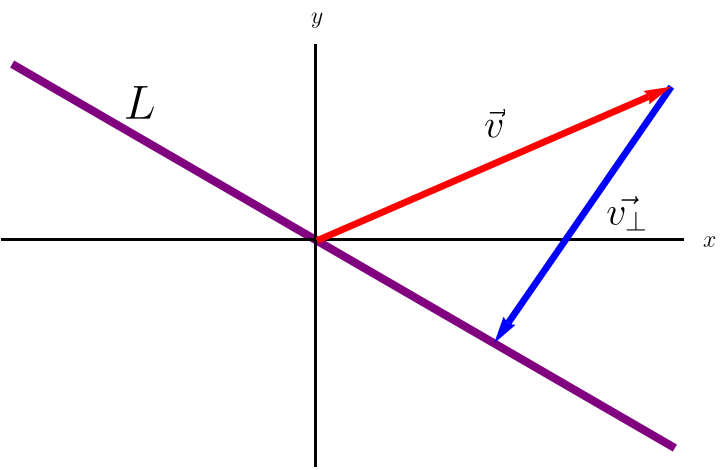
\includegraphics{misc/titlepage.png}
        \end{figure}
        \vfill
        
        \small
        by Louis Meunier
        
        \href{https://notes.louismeunier.net}{\color{violet}{notes.louismeunier.net}}
        
    \end{center}
\end{titlepage}


{
  \hypersetup{linkcolor=violet}
  \tableofcontents
}
\newpage
\pagestyle{mypage}
\section{Unit 1}
\subsection{Solving Linear Systems}
\subsubsection{Algebraically vs Geometrically}
Consider a set of linear equations, $a_1 x+b_1 y = c_1$ and $a_1 x+b_2 y = c_2$. Solving this should be fairly straightforward:
\begin{itemize}
    \item Isolate one variable in one of the equations
    \item Substitute said variable in the second equation
    \item Solve for second variable
    \item Plug in solution to second variable in either original equation to find the other variable
\end{itemize}

Doing this reveals one of two things: either the system is consistent, or inconsistent:

\begin{itemize}\label{list:solntypes}
    \item \textbf{Consistent}: a solution to the system exists. This can either be:
    \begin{itemize}
        \item \textbf{A unique solution} (Fig. \ref{fig:uniquesolutions})
        \item \textbf{Infinite solutions} (Fig. \ref{fig:infinitesolutions})
    \end{itemize}
    \item \textbf{Inconsistent}: no solution to the system exists (Fig. \ref{fig:nosolutions})
\end{itemize}

Being able to recognize when these particular circumstances occurs is essential.

Graphically, the differences between these are also very noticeable (see figures  \ref{fig:uniquesolutions}, \ref{fig:infinitesolutions}, and \ref{fig:nosolutions}.)

\begin{figure}[!ht]%
    \centering
    \subfloat[\centering Two equations with a unique solution]{{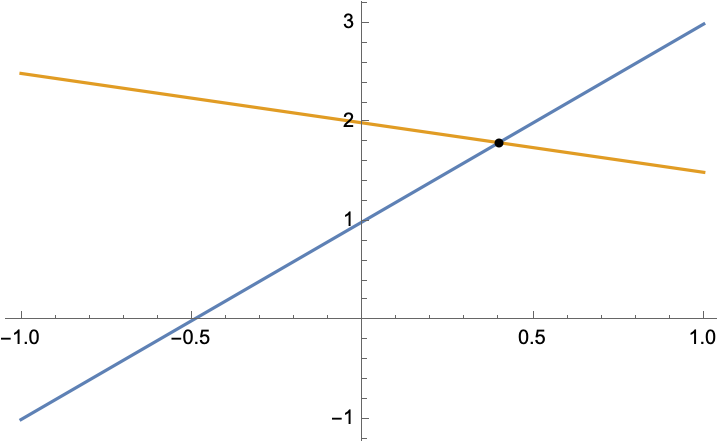
\includegraphics[width=6.5cm]{misc/twoequationsuniquesolution.png} }}%
    \qquad
    \subfloat[\centering Three equations with a unique solution]{{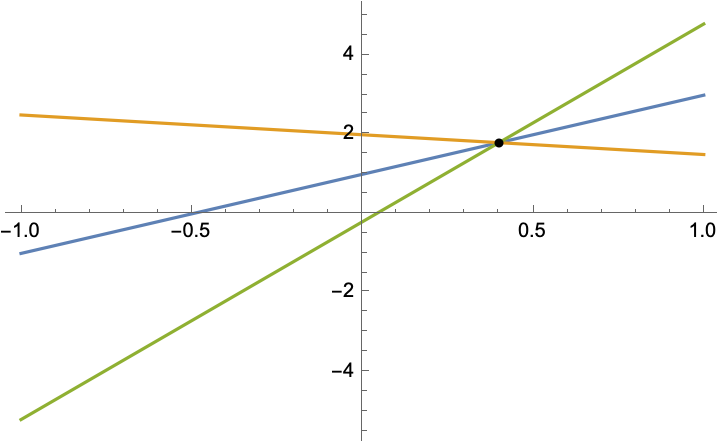
\includegraphics[width=6.5cm]{misc/threeequationsuniquesolution.png} }}%
    \caption{Unique solutions}
    \label{fig:uniquesolutions}%
\end{figure}

\begin{figure}[!ht]
    \centering
    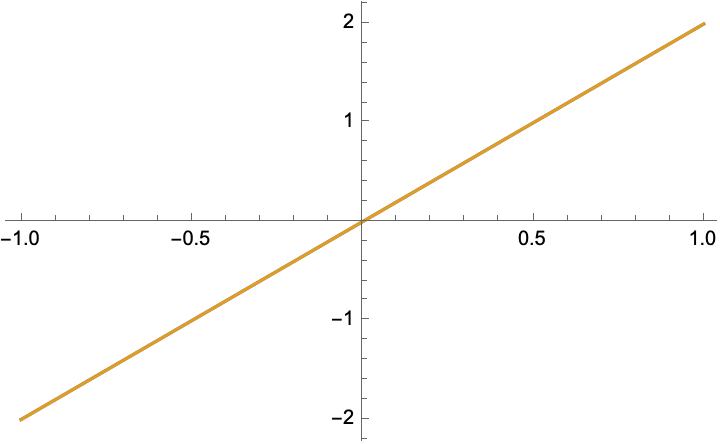
\includegraphics[width=6.5cm]{misc/infinitesolutions.png}
    \caption{Any number of equations with infinite solutions (always intersecting)}
    \label{fig:infinitesolutions}
\end{figure}

\begin{figure}[!ht]%
    \centering
    \subfloat[\centering Two equations with no solution]{{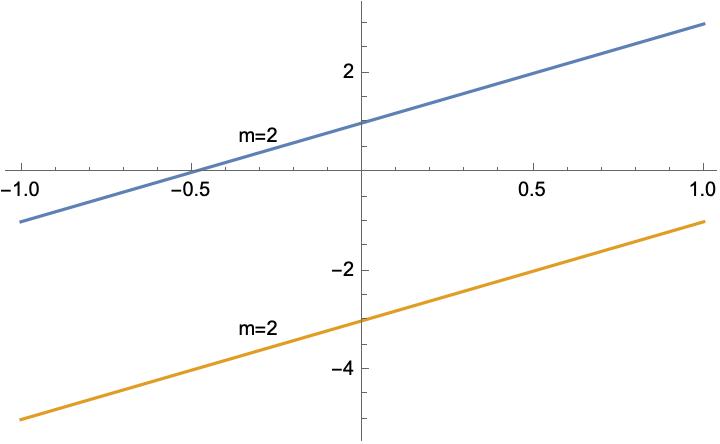
\includegraphics[width=6.5cm]{misc/twoequationsnosolution.png} }}%
    \qquad
    \subfloat[\centering Three equations with no solution]{{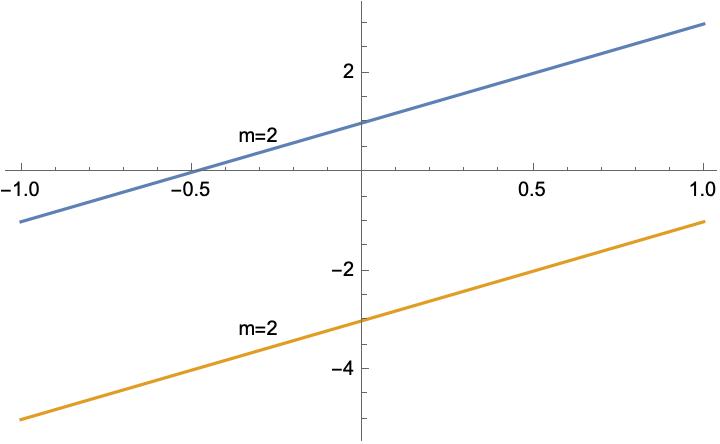
\includegraphics[width=6.5cm]{misc/twoequationsnosolution.png} }}%
    \caption{No solutions}
    \label{fig:nosolutions}%
\end{figure}

\subsubsection{Gaussian Elimination}
Although the procedure described above is fine for smaller equations, it can often become cumbersome. Using the concept of Gaussian Elimination, you can not only more easily solve systems of linear equations, but also determine patterns in said systems more easily.

To begin, create an \textbf{augmented matrix} of the system. This involves a \textbf{coefficient matrix} on the left, and the augmented part on the right.

The \textbf{coefficient matrix} has a row representing each equation, and each column representing the coefficients belonging to each individual variable in the system.

The \textbf{augmented matrix} contains each of the corresponding constants that the rows sum up to.

For example, the system

\begin{equation}
\begin{split}
    x + 2y - z &= 1\\    
    2x -3y + z &= 4\\
    y + 2z &= 0\\
\end{split}
\end{equation}

becomes

\[
    \begin{array}[t][{@{}ccc|c@{}}]
     1 & 2 & -1 & 1 \\
     2 & -3 & 1 & 4 \\
     0 & 1 & 2 & 0 \\
    \end{array}\
\]

Note that even though there is no $x$ in the third equation, its coefficient must still be represented (as a 0).

\subsubsection{rref}
When working with augmented matrices, there are a number of possible operations that can be used to reach the "end goal": \textbf{the row reduced echelon form (rref)}. An rref is achieved when:

\begin{itemize}
    \item The first non-zero term in each row (aka the \textbf{leading 1}) is a 1, and there are zeroes above and below it.
    \item The leading 1 in any row is to the right of the leading 1 above (\textit{this creates the typical staircase form}).
    \item Any rows with all zeros in the coefficient matrix are at the bottom.
\end{itemize}

A (very simple) rref matrix could look like this:

\[
    \begin{array}[t][{@{}ccc|c@{}}]
     1 & 0 & 0 & 1 \\
     0 & 1 & 0 & 4 \\
     0 & 0 & 1 & 0 \\
    \end{array}\
\]

To be clear: not all matrices will result in a nice, orderly pattern as this; most won't.

To get to this point at all, you must manipulate the matrix using certain operations:

\begin{itemize}
    \item Switch rows
    \item Add a multiple of one row to another
    \item Multiply a row by a constant
\end{itemize}

Note that all of these operations work on rows; attempting to manipulate columns will result in a wrong answer. 

\subsubsection{Determining Solutions from rref}

Given any rref matrix, you should be able to tell how many solutions a system has (and, by extension, what they are). The following examples should reveal some patterns in determining the number of solutions for any matrix:

\begin{itemize}
    \item 
    $
    \begin{array}[t][{@{}ccc|c@{}}]
     1 & 0 & 0 & c_1 \\
     0 & 1 & 0 & c_2 \\
     0 & 0 & 1 & c_3 \\
    \end{array}\
    $
    
    This system has \textbf{one unique solution}: when $x = c_1, y = c_2$ and $z = c_3$. This comes from the fact that each column represents a variable; thus, you can read the first row as $1*x+0*y+0*z = c_1$. The same idea applies for the rest of the rows.
    \item 
    $
    \begin{array}[t][{@{}ccc|c@{}}]
     1 & 0 & 0 & c_1 \\
     0 & 1 & 0 & c_2 \\
     0 & 0 & 0 & c_3 \neq 0 \\
    \end{array}\
    $
    
    This system has \textbf{no solutions}: in the final row is stating that $0*x+0*y+0*z \neq 0$, which is impossible. Thus, no solution to the system exists that would fulfil this requirement.
    \item 
    $
    \begin{array}[t][{@{}ccc|c@{}}]
     1 & 0 & 0 & c_1 \\
     0 & 1 & 0 & c_2 \\
     0 & 0 & 0 & 0 \\
    \end{array}\
    $
    
    This system has \textbf{infinite solutions}: in now row is there any restriction on the value of $z$. Thus, while $x = c_1$ and $y = c_2$, $z$ can be any real number. When this happens, $z$ is called a \textbf{"free variable"}. 
     
    In rref matrices of the following form, you can also have variables that are reliant on the value of free variables. 
     
     $$
    \begin{array}[t][{@{}ccc|c@{}}]
     1 & 0 & 0 & c_1 \\
     0 & 1 & 1 & c_2 \\
     0 & 0 & 0 & 0 \\
    \end{array}\
    $$
    
    In this case, $x = c_1$ and $y = c_2 - z$, where $z$ is free. It should be noted that you could also rewrite this as $z = c_2 - y$, in which case $y$ would be the free variable. Either way of writing it, there is one free variable.
\end{itemize}

There are many other forms, of varying complexity, that rrefs can have as well. However, following these simple patterns will make it fairly straightforward to determine the solutions in any situation.

\subsubsection{Representing Solutions}

As above, you can write the solutions to a system as $x = ..., y = ..., z = ...$. However, a more "standard" way, which will also make certain manipulations easier later, is:

\[
    \begin{bmatrix}
     x \\
     y \\
     z \\
    \end{bmatrix} 
    = 
    \begin{bmatrix}
     c_1 \\
     c_2 \\
     c_3 \\
    \end{bmatrix}
\]

Or, if there is a free variable: 
\[
    \begin{bmatrix}
    x \\
    y \\ 
    z \\
    \end{bmatrix}
    = 
    \begin{bmatrix}
    c_1 \\
    c_2 \\
    t \\
    \end{bmatrix}
    , t \in \real
\]

\subsubsection{Rank}

The \textbf{rank} of a matrix is the number of leading ones in the rref of that matrix. You can similarly say that the rank is equal to the number of columns of that matrix minus the number of free variables (though this way of thinking is more relevant later).

If a matrix has a rank equal to its number of columns, then the system of equations it represents is consistent and has a unique solution.

\subsection{Spans}
Before proceeding, we need to define a few concepts to analyze solutions and describe vectors and matrices in new ways.

A \textbf{linear combination} of the vectors $\Vec{v_1}, \Vec{v_2}, ..., \Vec{v_n}$ is an expression $c_1 \Vec{v_1} + c_2 \Vec{v_2} + ... + c_n \Vec{v_n}$, where $c_1, c_2,...,c_n \in \real$. In "simpler" terms, it is a sum of multiples of the vectors involved. 

A \textbf{span} of vectors is all possible linear combinations of a set of vectors, represented by the notation $span(\Vec{v_1}, \Vec{v_2}, ..., \Vec{v_n})$.

Spans can also be rewritten as a set; $span(\Vec{v_1}, \Vec{v_2}) = {c_1 \Vec{v_1} + c_2 \Vec{v_2}, c_1, c_2 \in \real}$. Being able to switch between these two forms will be important for later. 

Another important concept is being able to determine if a vector exists in a particular span; say, does the vector $\Vec{v}$ exist in $span(\Vec{x}, \Vec{y})$? This is the equivalent of asking whether a particular vector can be reached by summing multiples of a set of other vectors. Based on our "alternative" form of writing a span, we can say:

$$
\Vec{v} \stackrel{?}{\in} span(\Vec{x}, \Vec{y})={c_1\Vec{x} + c_2\Vec{y}, c_1,c_2 \in \real}
$$

Thus, we can say $\Vec{v} = c_1 \Vec{x} + c_2 \Vec{y}$. If and only if $c_1$ and $c_2$ exist can we say that $\Vec{v}$ is in $span(\Vec{x}, \Vec{y})$.


\subsection{Linear Relations}
Piggybacking off the ideas of linear combinations earlier, we can define a \textbf{linear relation} of vectors $\Vec{v_1}, \Vec{v_2}, ..., \Vec{v_n}$ as an equation of the form $c_1 \Vec{v_1} + c_2 \Vec{v_2} + ... + c_n \Vec{v_n} = \Vec{0}$.

If you can solve this equation where at least on $c_n$ is \textit{N
OT} 0, then this is called a \textbf{non-trivial linear relation}. Otherwise, if the only possible solution occurs when all $c_n$'s are 0, then this is a \textbf{trivial linear relation}.

From this, we can state yet another definition to describe vectors; \textit{linear (in)dependence}. A set of vectors can be described as \textbf{linearly independent} if the only linear relation between them that exists is the trivial one; conversely, a set of vectors are \textbf{linearly dependent} if a non-trivial linear relation exists.

Its helpful to think about this logically: if a set of vectors are \textit{dependent}, then one (or more) of the vectors relies on the one (or more) of the others. In more "mathematical" terms, this means that vectors in the set can be created from a sum of different multiples of others vectors in said set. This, on the other hand, is impossible between \textit{independent} vectors.

For example: is the vector $\begin{bmatrix}
1\\
2\\
\end{bmatrix}$ in $span(\begin{bmatrix}
-4\\
-5
\end{bmatrix}, \begin{bmatrix}
1\\
1\\
\end{bmatrix})$? If this were true, then we should be able to say that:

$$c_1 \twodmatrix{1}{1} + c_2 \twodmatrix{-4}{-5} = \twodmatrix{1}{2}, c_1, c_2 \in \real$$

$c_1$ and $c_2$ are, clearly, just \textit{scalars} of their respective vectors. As such, we can rewrite:

\begin{equation}
    \begin{split}
        \twodmatrix{c_1}{c_1} + \twodmatrix{-4 c_2}{-5 c_2} &= \twodmatrix{1}{2}\\
        \twodmatrix{c_1 - 4 c_2}{c_1 - 5 c_2} &= \twodmatrix{1}{2}
    \end{split}
\end{equation}

It should (hopefully) be clear that this is simply a system of linear equations, where $c_1$ and $c_2$ are the unknowns!

$$c_1 - 4 c_2 = 1; c_1 - 5 c_2 = 2$$

From here, we can simply use Gaussian elimination to see whether or not a solution does exist:

\[
    \begin{array}[t][{@{}cc|c@{}}]
     1 & -4 & 1 \\
     1 & -5 & 2 \\
    \end{array}\
    \Rightarrow
    \begin{array}[t][{@{}cc|c@{}}]
     1 & 0 & -3 \\
     0 & 1 & -1 \\
    \end{array}\
\]

Therefore, $c_1 = -3$ and $c_2 = -1$; as this system is consistent, then the vector is indeed in the span.

When working with spans of a number of vectors, it is important to be able to rewrite spans with as few vectors as possible; this is called the \textbf{basis} of the set. With more notation, we can say that the vectors $v_1, v_2, ..., v_n$ of set $V$ are a \textit{basis} of $V$ if they both \textit{span} $V$ and are \textit{linearly independent}. 

The first requirement here should make intuitive sense; if a set of vectors doesn't span $V$, then of course it can't represent it fully. 
The second requirement takes care of the "as few vectors as possible" part; if the opposite were true, and the vectors were linearly dependent, then one or more of the vectors could be represented by vectors already existing in the set.

Using the basis, we can then define the \textbf{dimension} of a set; the number of vectors in the \textit{basis} of the set.


\subsection{Subspaces}

A \textbf{subspace} of $\real^N$ is a non-empty set of vectors in $\real^N$, that can be described as a span of vectors. These two terms can often be interchanged, but be careful when you do so.

Formally, a subspace, $V$, must have the following properties:

\begin{enumerate}
    \item \textbf{Closed under scalar multiplication:} if $\Vec{u} \in V$, then $k\Vec{u} \in V$ for any scalar $k \in \real$ 
    \item \textbf{Closed under addition:} if $\Vec{v}, \Vec{w} \in V$, then $\Vec{v} + \Vec{w} \in V$.
\end{enumerate}

The concepts of bases and dimension similarly apply to subspaces, with the same rules.

\subsection{Standard Basis Vectors}
The standard basis vectors of $\real^n$ are written as $\Vec{e_i}$, with $i$ from $1$ to $n$, where the vector is made up of all 0's and a $1$ in the $i$th row. For example, the standard basis vectors $\real^2$ are $\Vec{e_1} = \twodmatrix{1}{0}, \Vec{e_2} = \twodmatrix{0}{1}$.

These standard basis vectors are, hopefully clearly, linearly independent; that is why they are called the "basis" after all. They will be helpful to use later on.

\subsection{Matrix-Vector Multiplication}
Being able to multiple a matrix by a vector has a large number of applications that are important to understand. We can approach defining matrix multiplication in a few ways.

\subsubsection{Column View}
Given a matrix $A$ and a vector $\Vec{x}$:

\[
A\Vec{x} = \begin{bmatrix}
&| &| & &|\\
&\Vec{c_1} &\Vec{c_2} &... &\Vec{c_n}\\
&| &| & &|\\
\end{bmatrix}\begin{bmatrix}
x_1\\
x_2\\
...\\
x_n\\
\end{bmatrix}=x_1 \Vec{c_1} + x_2 \Vec{c_2} + ... + x_n \Vec{c_n}
\]
 
In other words, this is defining the product of a matrix and vector as a linear combination of the columns of the matrix. It should be noted that this works by treating each column of the matrix $A$ as a vector; this can be helpful in better visualizing this operation.

\subsubsection{Row View}
Given a matrix $A$ and a vector $\Vec{x}$:

\[
A\Vec{x} = \begin{bmatrix}
&- & \Vec{r_1} &-\\
&- & \Vec{r_2} &-\\
& & ... &\\
&- & \Vec{r_m} &-\\
\end{bmatrix}\Vec{x}=\begin{bmatrix}
\Vec{r_1} \cdot \Vec{x}\\
\Vec{r_2} \cdot \Vec{x}\\
...\\
\Vec{r_m} \cdot \Vec{x}\\
\end{bmatrix}
\]

Note that "$\cdot$" represents a \textit{dot product}: this is the operation involving multiplying each element in one vector by the corresponding element in another vector.

Note that, conversely to above, this way of viewing the operation involves treating each row of $A$ as an individual matrix.

Deciding which "view" to use when is, often, very subjective to the particular situation. However, it should be noted that \textit{the result is the same no matter which view you take.}

\subsection{Linear Transformations}
A \textbf{linear transformation} $T: \real^n \to \real^m$ is a function that:
\begin{enumerate}
    \item \textbf{preserves vector addition}: $T(\Vec{x}+\Vec{y}) = T(\Vec{x}) + T(\Vec{y})$ for all $\Vec{x}, \Vec{y}$
    \item \textbf{preserves scalar addition}: $T(c \Vec{x}) = c T(\Vec{x})$ for all $\Vec{x}$ and $c \in \real$
\end{enumerate}

Linear transformations are often described by a matrix $A$, which \textit{induces} said linear transformation. In other terms:

\[
T: \real^n \to \real^m = T(\Vec{x}) = A\Vec{x}
\]

This matrix $A$ must be an $m$ x $n$ matrix in order for this formula to make sense.

\subsubsection{Determining Linear Transformations}
In order to figure out the linear transformation $T$ of any vector, you must know the $T(\Vec{x})$ of as many linearly independent $\Vec{x}$'s as there are columns in the matrix $A$. If you know, or are able to determine, the $T$ of the standard basis vectors of $A$, it is far easier to determine the linear transformation of any vector, thanks to the properties of linear transformations:
\[
T(\Vec{x}) = T(c_1 \Vec{e_1} + c_2 \Vec{e_2} + ...) = c_1 T(\Vec{e_1}) + c_2 T(\Vec{e_2}) + ...
\]

Using this same pattern, we can rewrite the $T$ of any vector $\Vec{x}$ as a sum of multiples of the $T$ of the standard basis vectors. 

\subsubsection{Geometric Linear Transformations}
Linear transformations can be visualized as a number of geometrical transformations; representing these in two dimensions makes it easiest to comprehend, but the same concepts are applicable to an arbitrary number of dimensions.

Say $T(\Vec{x}) = A\Vec{x}$, consider the following transformations on the standard basis vectors $\Vec{e_1}$ and $\Vec{e_2}$ of $\real^2$ (see figure \ref{fig:beforetransform}):

\begin{figure}[!ht]
    \centering
    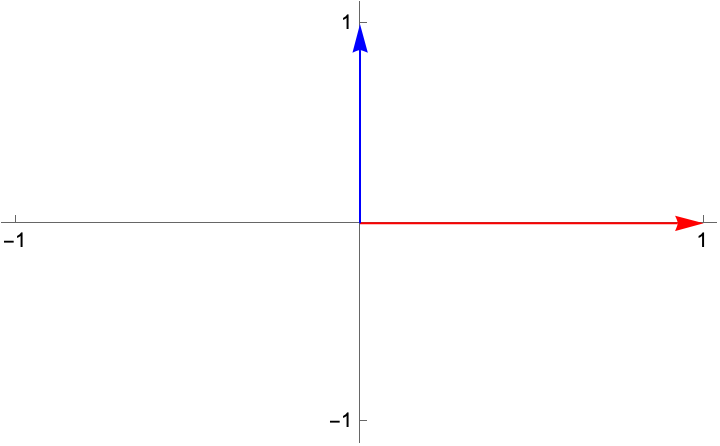
\includegraphics[width=8cm]{misc/beforetransformation.png}
    \caption{$\Vec{e_1}, \Vec{e_2}$ before any transformation}
    \label{fig:beforetransform}
\end{figure}
\newpage
\begin{itemize}
    \item $A = \begin{bmatrix}
    -1 &0\\
    0 &1\\
    \end{bmatrix}$ 
    
    $T(\Vec{e_1}) = \twodmatrix{1}{0} \twobytwomatrix{-1}{0}{0}{1} = \twodmatrix{-1}{0}, T(\Vec{e_2}) = \twodmatrix{0}{1} \twobytwomatrix{-1}{0}{0}{1} = \twodmatrix{0}{1}$
    
    \begin{figure}[!ht]
        \centering
        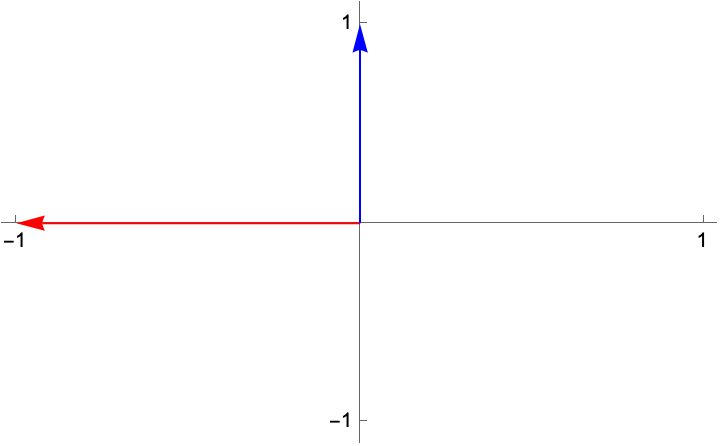
\includegraphics[width=8cm]{misc/reflectionoveryaxis.png}
        \caption{Reflection of $\Vec{e_1}, \Vec{e_2}$ over the y-axis}
    \end{figure}
    
    \item $A = \twobytwomatrix{0}{1}{1}{0}$ 
    
    $T(\Vec{e_1}) = \twodmatrix{1}{0} \twobytwomatrix{0}{1}{1}{0} = \twodmatrix{0}{1}, T(\Vec{e_2}) = \twodmatrix{0}{1} \twobytwomatrix{0}{1}{1}{0} = \twodmatrix{1}{0}$
    
    \begin{figure}[!ht]
        \centering
        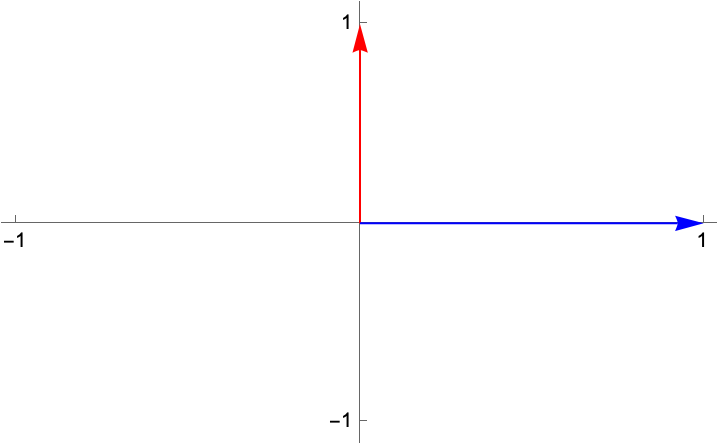
\includegraphics[width=8cm]{misc/reflectionoveryequalsx.png}
        \caption{Reflection of $\Vec{e_1}, \Vec{e_2}$ over $y=x$}
    \end{figure}
    \newpage
    \item $A = \twobytwomatrix{1}{-1}{0}{1}$ 
    
    $T(\Vec{e_1}) = \twodmatrix{1}{0} \twobytwomatrix{1}{-1}{0}{1} = \twodmatrix{1}{0}, T(\Vec{e_2}) = \twodmatrix{0}{1} \twobytwomatrix{1}{-1}{0}{1} = \twodmatrix{-1}{1}$
    
    \begin{figure}[!ht]
        \centering
        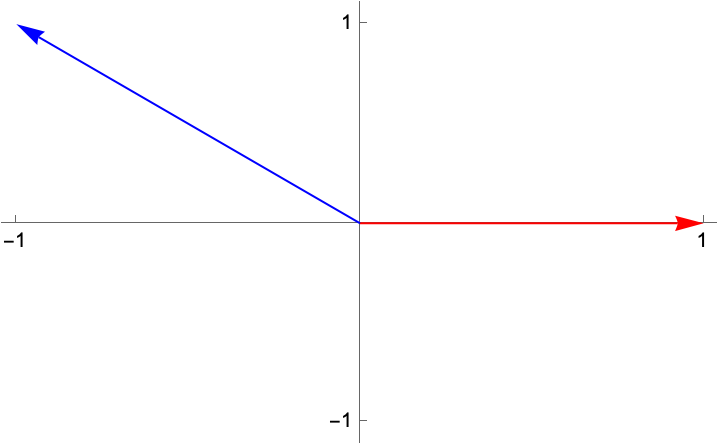
\includegraphics[width=8cm]{misc/horizontalshear.png}
        \caption{Shear of $\Vec{e_1}, \Vec{e_2}$ towards left}
    \end{figure}
    
    \item $A = \twobytwomatrix{0}{-1}{1}{0}$ 
    
    $T(\Vec{e_1}) = \twodmatrix{1}{0} \twobytwomatrix{0}{-1}{1}{0} = \twodmatrix{0}{1}, T(\Vec{e_2}) = \twodmatrix{0}{1} \twobytwomatrix{0}{-1}{1}{0} = \twodmatrix{-1}{0}$
    
    \begin{figure}[!ht]
        \centering
        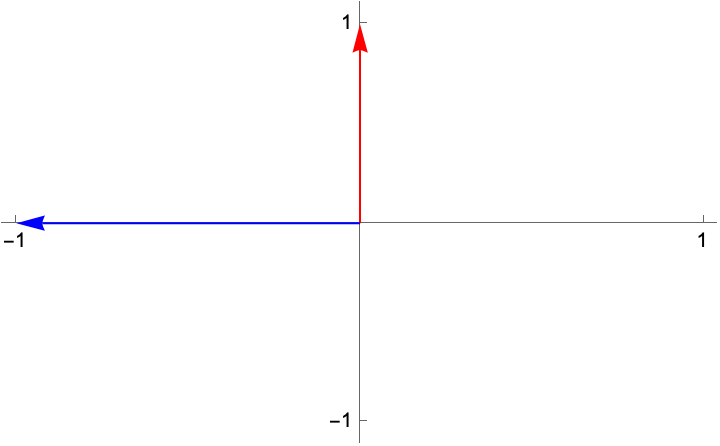
\includegraphics[width=8cm]{misc/rotationaboutorigin.png}
        \caption{Rotation counter-clockwise of $\Vec{e_1}, \Vec{e_2}$ about the origin}
    \end{figure}
\end{itemize}

In these transformations, finding the effect on the standard basis vectors is typically quite simple, while finding the transformation for any random vector can be quite difficult. So, we can instead use the rules of linear transformations to find the effect on any vector in terms of its ratio to the standard basis vectors.

\subsubsection{A Quick Look at Projections}

If a plane $P$ passes through the origin in $\real^n$, any vector $\Vec{x} \in \real^n$ can be written as $\Vec{x}^{\parallel} + \Vec{x}^{\perp}$, where $\Vec{x}^{\parallel}$ is a vector \textit{in the plane} $P$ and $\Vec{x}^{\perp}$ is a vector \textit{perpendicular} to $P$. This can be defined as a linear transformation $\text{proj}_P:\real^n \to \real^n = \text{proj}_P(\Vec{x}) = \Vec{x}^{\parallel}$

\section{Unit 2}
\subsection{Images and Kernels}

For a matrix $A$, we can define the following (useful) subsets:

\begin{itemize}
    \item \textbf{kernel:} aka null space, written ker$(A)$, is the set of vectors $\Vec{x}$ where $A\Vec{x} = \Vec{0}$.
    
    \item \textbf{image:} written im$(A)$, the set of vectors $\Vec{y}$ where $\Vec{y} = A\Vec{x}$. This is more commonly known as the "range" for functions.
\end{itemize}

You can solve for ker$(A)$ by simply augmenting $A$ by $\Vec{0}$. The image of $A$ is simply the span of the columns of $A$ (which is fairly simple to prove, so it won't be shown here).

\subsubsection{Rank-Nullity Theorem}

A useful pattern to keep in mind is that the rank of an rref matrix is equal to the dimension of the image, and the number of free columns in the rref matrix is equal to the dimension of the kernel.

This pattern leads to what is called the \textbf{Rank-Nullity Theorem}.

\subsection{Matrix Algebra}

Similarly to processes described earlier for performing algebraic operations between vectors and vectors, as well as vectors and matrices, it is also possible to perform a number of operations between matrices. However, there are some very specific limitations and rules that must be followed that can make said operations rather unintuitive if viewed as purely extensions of the operations performed between numbers, for instance.

\begin{itemize}
    \item \textbf{Matrix times scalar}
    
    Multiplying a matrix $A$ times a scalar $k$ is very similar to multiplying a vector times a scalar:
    
    \begin{equation}
        \begin{split}
            kA &= k\twobytwomatrix{A_{1a}}{A_{2a}}{A_{1b}}{A_{2b}}\\
            &= \twobytwomatrix{k A_{1a}}{k A_{2a}}{k A_{1b}}{k A_{2b}}\\
        \end{split}
    \end{equation}
    
    \item \textbf{Matrix plus matrix}
    
    Adding together two matrices (say $A$, a $n$ x $m$, and $B$, a $p$ x $q$) requires certain restrictions on the dimensions of the affected matrices, just as in vector addition. In this case, $n=p$ and $m=q$:
    
    \begin{equation}
        \begin{split}
            A + B &= \begin{bmatrix}
            A_{1a} & A_{2a} & A_{3a}\\
            A_{1b} & A_{2b} & A_{3b}\\
            \end{bmatrix} + \begin{bmatrix}
            B_{1a} & B_{2a} & B_{3a}\\
            B_{1b} & B_{2b} & B_{3b}\\
            \end{bmatrix}\\
            &= \begin{bmatrix}
            A_{1a}+B_{1a} & A_{2a}+B_{2a} & A_{3a}+B_{3a}\\
            A_{1b}+B_{1b} & A_{2b}+B_{2b} & A_{3b}+B_{3b}\\
            \end{bmatrix}
        \end{split}
    \end{equation}
    \item \textbf{Matrix times matrix}
    
    In order to multiply two matrices (say $A$, a $n$ x $m$, and $B$, a $p$ x $q$), another set of restrictions apply, that may be a little trickier to interpret. Say you're finding $AB$; here, $m = p$, and the resulting matrix is an $n$ x $q$ matrix. 
    
    When multiplying two matrices, you can imagine the first matrix being multiplied by each of the columns of the second matrix, treating each column as a vector. The result of each vector-matrix multiplication becomes the corresponding column of the resulting matrix. Given these steps, the above restrictions should hopefully make more intuitive sense.
    
    It should also be clear from these steps that \textbf{multiplying matrices is not commutative;}
    
    \begin{equation}
        \begin{split}
            &A = \begin{bmatrix}
            1 & 0 & 2 \\
            2 & -2 & 1 \\
            3 & 1 & 0 \\
            \end{bmatrix}\\
            &B = \begin{bmatrix}
            -1 & 3\\
            2 & 0\\
            1 & 1\\
            \end{bmatrix} = \begin{bmatrix}
            \Vec{b_1} & \vec{b_2}\\
            \end{bmatrix}\\
            AB &= \begin{bmatrix}
            A\Vec{b_1} & A\Vec{b_2}\\
            \end{bmatrix}\\
            &= \begin{bmatrix}
                (-1*2+2*0+1*2) & (3*1 + 0*0 + 1*2) \\
                ... & ...\\
                ... & ...\\
            \end{bmatrix}\\
            &= \begin{bmatrix}
                1 & 5\\
                -5 & 7\\
                -2 & 9\\
            \end{bmatrix}
        \end{split}
    \end{equation}
    
    Doing $BA$, on the other hand, would result in a $2$ x $3$ matrix, which, naturally, would not be equal to the product of $AB$.
    
    \item \textbf{Identity Matrix}
    
    While not exactly an algebraic operation, its important to note that the notation $I$ is often used to denote the \textbf{identity matrix}, a matrix such that $AI = A$. $I$ is essentially a rref matrix with the same number of leading ones as columns. Example:
    
    \[
    I_{2} = \begin{bmatrix}
    1 & 0\\
    0 & 1\\
    \end{bmatrix}
    \]
    
    \item \textbf{Solving for a matrix given its product}
    
    If you are given a matrix $A$ and the product of $A$ with an unknown matrix $B$, you can find $B$ fairly easily using a similar idea as discussed above; by treating each column of $B$ as a vector.
    
    \begin{equation}
    \begin{split}
        AB = \begin{bmatrix}
        -1 & 0 \\
        4 & 5 \\
        0 & 1\\
        \end{bmatrix}B &= \begin{bmatrix}
        -1 & -1 & 0\\
        9 & -1 & -10\\
        1 & -1 & -2\\
        \end{bmatrix}\\
    \end{split}
    \end{equation}
    
    Treating each column of $B$ as a vector ($\vec{b_1}$, etc), we can write the product of each column of $B$ equal to the corresponding column of the product of $A$ and $B$:
    
    \begin{equation}
    \begin{split}
        \vec{b_1}A = \begin{bmatrix}
        -1\\
        9\\
        1\\
        \end{bmatrix}, ...
        \end{split}
    \end{equation}
    
    Finding the vector that multiplies to a matrix to produce a given vector has already been discussed above, so the steps from here (creating an augmented matrix and solving for each component of $\vec{b_n}$) should be clear. However, we can make the work a little easier by simply creating an augmented matrix of $A$ augmented by the product of $AB$:
    
    \begin{equation}
        \begin{split}
             \begin{array}[t][{@{}cc|ccc@{}}]
                 -1 & 0 & -1 & -1 & 0 \\
                 4 & 5 & 9 & -1 & -10 \\
                 0 & 1 & 1 & -1 & -2 \\
                \end{array}\
        \end{split}
    \end{equation}
    
    All row operations to the left hand side of this matrix would be the same no matter the augmented side, so this technique should (hopefully) seem intuitively correct.
\end{itemize}

\subsection{Compositions}

Recall that we can describe a linear transformation $T(\vec{x})$ as a matrix $A$ times the vector $\vec{x}$. However, what if we want to perform two (or more!) linear transformations, one after another? Rather than simply performing said linear transformations one after another, we can use the concept of \textbf{compositions}.

For instance, say we want $T$ composed with $S$. This can be written as follows, given $T(\vec{x}) = A\vec{x}$ and $S(\vec{x}) = B\vec{x}$:

\begin{equation}
    \begin{split}
        T \circ S &= T(S(\vec{x}))\\
        &= T(B\vec{x})\\
        &= A(B\vec{x})\\
    \end{split}
\end{equation}

This composition, just like the functions is composes, is linear. This can be proved using aforementioned definitions, but should also make intuitive sense. 

Another common question is how to find the single matrix, say $C$, that induces the composition. As shown above, a composition is simply a vector multiplied by a number of matrices, so we can find $C$ by simply multiplying the matrices involved (in this case, $A$ and $B$) using the method described earlier.

Note that, since this is essentially just matrix-matrix multiplication, \textbf{order matters}.

\subsubsection{Transformation Inverses}

Given a particular transformation $\vec{y} = T(\vec{x})$, we know we can describe it as $\vec{y}=A\vec{x}$. However, it is very helpful to be able to describe its inverse, $T^{-1}(\vec{x}) = S(\vec{y}) = \vec{x}$. By a natural extension, we should be able to find a matrix $B$ such that $B \vec{y} = \vec{x}$. Below will describe strategies for finding $B$ for a number of transformations, and later how to generalize said strategies to any matrix $A$.

First, let's look at a number of common linear transformations, and how to determine their inverses; if possible.

\begin{itemize}
    \item \textbf{Reflections}
    
    \[
    T(\vec{x}) = ref_L(\vec{x})
    \]
    
    How do we reflect a vector back over to where it started? Well, as the question almost answers by itself, you simply reflect it again. As such, we can say $T^{-1} = T$.
    
    \item \textbf{Rotations}
    
    \[
    T(\vec{x}) = rot(\vec{x})
    \]
    
    Say our transformation rotates a vector $\vec{x}$ by an angle $\Theta$ clockwise. To invert this, we can simply rotate it counterclockwise by $\Theta$, or, equivalently, clockwise by $-\Theta$.
    
    \item \textbf{Projections}
    
    \[
    T(\vec{x}) = proj_L(\vec{x})
    \]
    
    How can we invert a projection? Simply put: we can't! When a vector $\vec{x}$ is projected onto a line $L$, for instance, we lose information about the original $\vec{x}$, and thus have no way of returning to $\vec{x}$. Another way to interpret this is that $T(\vec{x})$ for any $\vec{x} \perp L$ equals $\vec{0}$, and thus it is impossible to go backwards to find any individual $\vec{x}$.
\end{itemize}

From these few examples, we can generalize the following: a transformation $T: \real^m \to \real^n$ is only invertible if for all \textit{outputs} $\vec{y} \in \real^n$ there exist a $\vec{x} \in \real^m$ such that $T(\vec{x}) = \vec{y}$ and $\vec{x}$ is unique.

We can think about this a little differently by considering $A$ such that $T(\vec{x})=A\vec{x} = \vec{y}$. Given our definition above, $A\vec{x}=\vec{y}$ must be consistent for any $\vec{y}$ if $T$ is invertible. As such, we can say that rref$(A)$ must have a leading one in each \textit{row}.

Further, we also require that $A\vec{x}=\vec{y}$ has a unique solution, so rref$(A)$ must also have a leading one in each \textit{column}. 

The only way that this is possible, to begin with, is that the number of columns of $A$ equals to the number of rows of $A$, and by extension, rref$(A) = I$. In other words, the matrix must be square.

\subsubsection{Inverting a Matrix}

As seen earlier in Unit 1, we can say that a transformation $T(\vec{x}) = A\vec{x} = \begin{bmatrix}
T(\vec{e_1}) & T(\vec{e_2})
\end{bmatrix}\vec{x}$. To find the inverse of $A$ ($A^{-1}$), we can say that $A^{-1} = \begin{bmatrix}T^{-1}(\vec{e_1}) & T^{-1}(\vec{e_2})\end{bmatrix}$.

We can say that $\vec{c_n} = T^{-1}(\vec{e_n})$, so $T(\vec{c_n}) = \vec{e_n}$. Thus, we can say that each $n$th column of matrix $A$ times some $\vec{c_n}$ equals $\vec{e_n}$. To find each $\vec{c_n}$ (ie, find each column of $A^{-1}$), we can therefore augment $A$ by the corresponding number of unit vectors; or, in other words, $I_n$.

For example, to invert $\begin{bmatrix} 3 & 2\\
7 & 5\\
\end{bmatrix}$, we write:

\begin{equation}
    \begin{split}
        \begin{array}[t][{@{}cc|cc@{}}]
             3 & 2 & 1 & 0\\
             7 & 5 & 0 & 1\\
            \end{array}&\\
    &=\begin{array}[t][{@{}cc|cc@{}}]
             1 & 0 & \vec{c_1} & \vec{c_2}\\
             0 & 1 & | & |\\
        \end{array}\\
    &=\begin{array}[t][{@{}c|c@{}}]
             I & A^{-1}\\
        \end{array}\\
    \end{split}
\end{equation}

\subsection{Bases and Coordinates}

\subsubsection{Introduction}
% this part is really wordy, maybe fix?
To understand the use of bases in linear algebra, consider the standard basis vectors, $\vec{e_1}, \vec{e_2}, ..., \vec{e_n}$. Any vectors in $R^n$ can thus be rewritten as a combination of these standard vectors ($c_1\vec{e_1} + c_2\vec{e_2} + ... + c_n\vec{e_n}$). However, consider a situation in which, say, "movements" are restricted to only a particular set of vectors (say $\vec{v_1}$ and $\vec{v_2}$) that aren't the standard basis vectors. 

While you can write these vectors, or any combinations of these vectors, as a combination of standard basis vectors, it can be easier to call these vectors as a new set of "basis vectors". We define this as $\mathfrak{B} = \{\vec{v_1}, \vec{v_2}\}$, ie $\mathfrak{B}$ is a basis of $\real^2$.

When writing about vectors in basis $\mathfrak{B}$, we use the notation $[y]_{\mathfrak{B}} = \begin{bmatrix}
    c_1\\
    c_2\\
\end{bmatrix}$ to indicate the coordinates of $\Vec{y}$ in the $\mathfrak{B}$ basis. This vector can thus, by extension, be represented as a linear transformation of the vectors in the basis $\mathfrak{B}$.

\subsubsection{Changing Bases}

To change a vector from one base to another, we can find a matrix $S$ such that $S[\vec{x}]_{\mathfrak{B}} = \vec{x}$, where $S$ is typically called the "change of basis matrix", in this case, changing base from $\mathfrak{B}$ to the standard basis.

Finding $S$ is fairly straightforward. We know that $S$ times each vector in $\mathfrak{B}$ must equal the corresponding standard basis vector, so we can write $S\vec{v_1} = \vec{e_1}$, $S\vec{v_2} = \vec{e_2}$, and so on. Therefore, $S$ simply equals the matrix of the vectors in $\mathfrak{B}$, ie $S = \begin{bmatrix}
    | & | & |\\
    \vec{v_1} & \vec{v_2} & ...\\
    | & | & |\\
\end{bmatrix}$.

To extend this, since we can say that $S[\vec{x}]_{\mathfrak{B}} = \vec{x}$, we can inversely say that $[\vec{x}_{\mathfrak{B}}] = S^{-1}\vec{x}$, so to find the matrix that changes bases in the opposite direction, we simply find the inverse of $S$. From here, this same rationale can be extended transform between any two bases in the same $\real^{n}$.

\subsubsection{Application to Transformations}

As noted earlier, we can define a linear transformation as a matrix $A$ such that $T(\vec{x}) = A\vec{x}$. With the added knowledge of bases, we can often more easily find the matrix of a transformation by carefully picking a basis for the transformation which makes the matrix easier to find.

To demonstrate this, take a transformation $T$ that projects vectors in $\real^{3}$ onto the plane $P$ defined by $3x_1+2x_2-5x_3=0$. To find a matrix $A$ such that $T(\vec{x}) = A\vec{x}$, we can create a basis $\mathfrak{B}$ of $R^{3}$ using vectors that make $A$ easy to compute.


For this particular case, we can define $\mathfrak{B} = \{\vec{v_1}, \vec{v_2}, \vec{v_3}\}$, where:

\begin{itemize}
    \item $\vec{v_1} = \begin{bmatrix}
        3\\
        2\\
        -5
    \end{bmatrix}$, since $T(\vec{v_1}) = 0$, as it is perpendicular to $P$

    \item $\vec{v_2} = \begin{bmatrix}
        0\\
        5\\
        2
    \end{bmatrix}$, since $T(\vec{v_2}) = \vec{v_2}$, as it lies along $P$

    \item $\vec{v_3} = \begin{bmatrix}
        5\\
        0\\
        3
    \end{bmatrix}$, since $T(\vec{v_3}) = \vec{v_3}$, as it also lies along $P$
\end{itemize}

To put it in more clear notation, we say that $[T(\vec{v_1})]_{\mathfrak{B}} = \vec{0}$, $[T(\vec{v_2})]_{\mathfrak{B}} = \begin{bmatrix}
0\\
1\\
0\\\end{bmatrix}$, and $[T(\vec{v_3})]_{\mathfrak{B}} = \begin{bmatrix}
    0\\
    0\\
    1\end{bmatrix}$; this step should make sense, as each vector denoted is the corresponding combination of vectors in $\mathfrak{B}$. Here, it should be clear that any vectors that that form a base of $\real^{3}$ could realistically have been used here, but these are clearly easier to work with.

    From here, we can define $B$, such that $B[\vec{v_1}]_{\mathfrak{B}} = [T(\vec{v_1})]_{\mathfrak{B}}$, simply enough as $B = \begin{bmatrix}
        0 & 0 & 0\\
        0 & 1 & 0\\
        0 & 0 & 1\\
    \end{bmatrix}$.

    From the previous section, we showed that $S^{-1}\vec{x} = [\vec{x}]_{\mathfrak{B}}$. Extending that to this linear transformation, we can recap our steps above using a number of matrices, as follows:

    \begin{equation}
        \begin{split}
            T(\vec{x}) &= A\vec{x}\\
            [T(\vec{x})]_{\mathfrak{B}} &= B[\vec{x}]_{\mathfrak{B}}\\
            [T(\vec{x})]_{\mathfrak{B}} &= B\red{S^{-1}}\vec{x}\\
            T(\vec{x})&= \red{S}BS^{-1}\vec{x}\\
            \implies A &= SBS^{-1}\\
        \end{split}
    \end{equation}

The final line above indicates a general process that can be used to find a matrix to represent any linear transformation, and while this process may seem initially more difficult that previously discussed methods, it has many advantages as well.

\subsection{Elementary Matrices}

Throughout these notes, the idea of "Gaussian elimination" and row reduction has been constantly discussed, with the concept of modifying the rows and columns of a matrix through a number of operations. \textbf{Elementary matrices} define matrices that, when multiplied to another matrix, execute these same row operations. These are typically denoted with an $E$.


\subsubsection{Types of Elementary Matrices}

Just as there a set number of possible row operations that we can perform on matrices, there are a corresponding number of elementary matrices that we can define to perform the equivalent transformations.

\begin{itemize}
    \item[\textbf{I}]: Row Interchanges
    
    This type of elementary matrix simply swaps rows of a matrix. For example, for a 2 by 3 matrix:


    \begin{equation}
        \begin{bmatrix}
            0 & 1 \\
            1 & 0\\
        \end{bmatrix} \begin{bmatrix}
            a & b & c\\
            p & q & r\\
        \end{bmatrix} = \begin{bmatrix}
            p & q & r\\
            a & b & c\\
        \end{bmatrix}
    \end{equation}

    The elementary matrix $\begin{bmatrix}
        0 & 1\\
        1 & 0\\
    \end{bmatrix}$ swaps the first and second rows, as shown. It should also be clear that there could be \textit{any number of columns in the matrix on the left}, and the elementary matrix would still perform the same operation.

    Finding the matrix to exchange rows for any dimension of matrix is fairly straightforward, as the matrix will only involve $0$'s and $1$'s in different positions.

    If we were to invert this operation, we can simply use the same elementary matrix again. Thus, in this case, $E = E^{-1}$; this can be verified by manually inverting $E$ as well, by using methods described earlier. 

    \item[\textbf{II}]: Row Multiplication

    To multiply a particular row (or rows) of a matrix by a constant, we can define another fairly simply elementary matrix that involves essentially all $1$'s and $0$'s again, except for the appropriate constant in the appropriate position. For instance, say we want to multiply the second row of the same matrix as above by $3$:

    \begin{equation}
        \begin{bmatrix}
            1 & 0 \\
            0 & 3\\
        \end{bmatrix} \begin{bmatrix}
            a & b & c\\
            p & q & r\\
        \end{bmatrix} =  \begin{bmatrix}
            a & b & c\\
            3p & 3q & 3r\\
        \end{bmatrix}
    \end{equation}

    To invert this operation, we have to divide the appropriate row by the same constant, or, more appropriately, multiply it by the inverse of the constant. Thus, $E^{-1} = E$ but with the constant inverted (fractional).

    \item[\textbf{III}]: Adding Multiples of Rows
    
    Adding a certain number of a row (or rows) to another row (or rows) of a matrix is, often, the most complicated to describe with an elementary matrix. However, with an example, it should hopefully be rather clear; so, to add twice the second row to the first row of a matrix, consider the following:

    \begin{equation}
        \begin{bmatrix}
            1 & 2 \\
            0 & 1\\
        \end{bmatrix} \begin{bmatrix}
            a & b & c\\
            p & q & r\\
        \end{bmatrix} =  \begin{bmatrix}
            a + 2p & b + 2q & c + 2r\\
            p & q & r\\
        \end{bmatrix}
    \end{equation}

    To invert this operation, we have to subtract the constant times the same row from the row involved. In this particular case, $E^{-1} = \begin{bmatrix}
        1 & -2\\
        0 & 1\\
    \end{bmatrix}$.
\end{itemize}

It should be noted that, in all these operations, the elementary matrix was invertible; and not only that, the inverted elementary matrix was also an elementary matrix in its own regard. If we want to invert such a matrix, we can either do so with typical methods (augmenting it by $I$) or by simply finding the logical inverse of the operation that the elementary matrix performs. 

It should be noted that you will often see problems with the following format, for some matrix $A$:

\begin{equation}
    E_5E_4E_3E_2E_1A
\end{equation}

While this may seem scary, since it is a whole lot of matrix-matrix multiplication, once you are able to determine what operation each $E_n$ performs, calculating this should be fairly straightforward. Simply find $A$ after $E_1$'s operations on performed on it, then after $E_2$ is performed on the result of that, etc..

\subsection{Distances}

% this sounds badly worded
Finding the distance between arbitrary figures in a particular space is very important in a number of applications. This section will cover the general trend for finding the distance between points, lines, and planes in $\real^{n}$.

\subsubsection{Point to Point}

\begin{figure}[!ht]
    \centering
    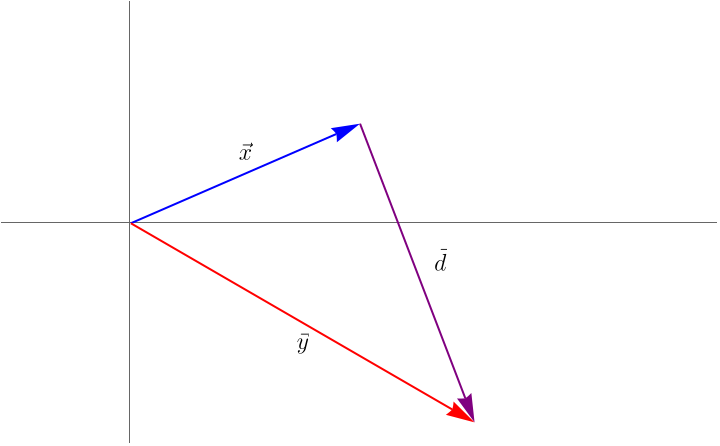
\includegraphics[width=8cm]{misc/vectordistance.png}
    \caption{Vector-vector distance}
    \label{fig:vectorvectordistances}
\end{figure}

Given two points, we can consider the point as the tip of a vector in the respective base (see figure \ref{fig:vectorvectordistances}). From here, the distance between the two vectors is clear: it is simply the length of the vector between the two points. If we consider two vectors $\vec{x}$ and $\vec{y}$, then we can write the distance vector $\vec{d}$ as:

$$\vec{x} + \vec{d} = \vec{y} \implies \vec{d} = \vec{y} - \vec{x}$$

From here, we simply find the length of $\vec{d}$, denoted as $\| \vec{d} \| $, using the Pythagorean theorem (and its higher-dimension extensions...):

$$\| \vec{d} \|  = \sqrt{d_1^2 + d_2^2 + ... + d_n^2}$$

\subsubsection{Point to Line}
% rephrase, a little confusing
Finding the distance between a point and a line (specifically, the shortest distance; this is really the only helpful one that should be found, as any point can be considered an infinite distance from a particular point on a line...) requires a little more intuitive and computation (though it can be simplified later). First, to understand how to find this shortest distance, we have to consider the properties of a particular point on the line in question that creates this shortest distance with our given point. Perhaps this is intuitive, but this point is the point on the line that forms a distance vector that is perpendicular to the line. 

% Consider a point $P = (a,b)$, a line $L$, a distance vector $\vec{d}$, in $\real^2$ (any base could work, but this is clearly the easiest to visualize), and the figure \ref{fig:pointtolinedistance}, as it is hard to visualize based off these words alone.

% add figure here

% standardize notation here - d'? d_\perp? etc
From the figure, it should be clear that if $\vec{d}$ is drawn anywhere else along the line $L$, it will be longer than if drawn perpendicular. You can visualize this as $\vec{d'}$ forming the hypotenuse of a triangle, with another side being $\vec{d_{\perp}}$; the hypotenuse is always the longest side of a triangle, and thus, $\vec{d'}$ would be longer than $\vec{d_{\perp}}$. 

As discussed in earlier sections, the projection of a vector perpendicular onto a particular line (or any space really, but a line in this case) is simply $\vec{0}$. As such, we can determine the vector $\vec{d}$ (and from here, naturally, finding its distance) by writing the linear transformation $T(\vec{x}) = proj_{L}\vec{x}$, finding the matrix $A$ that induces this transformation, and finding $\vec{d}$. 

\begin{equation}
    \begin{split}
        \vec{d}\perp L \implies T(\vec{d}) = \vec{0}, T(\vec{x}) = proj_L (\vec{x}) \\
        T(\vec{x}) = M\vec{x} \therefore M\vec{d} = \vec{0} \\
    \end{split}
\end{equation}

% add more here, this isn't very clear - better notation
Note that a very similar method can be used to find the distance between a point and a line that doesn't pass through the origin, by adding the distance from the line to the origin when computing the transformation. 

% add that you can use the known formula for calculating a projection, dot product over magnitude or w/e

% add section about plane to point; same thing, basically
\subsubsection{Point to Plane}

Finding the distance between a point and a plane is conceptually similar to above, but much harder to visualize. The general methods are as follows, given a plane $P$, that doesn't go through the origin, and a point $Q$ (ie the tip of a vector $\vec{Q}$):
\begin{itemize}
    \item Pick any point $R$ on the plane. Using this, we can define $\vec{Q} = \vec{R} + \vec{x}$, where $\vec{R}$ describes the vector with a point at $R$. Note that the important vector here is $\vec{x} ( = \vec{Q}-\vec{R})$.
    \item Define the distance vector $\vec{d}$ between $Q$ and $P$, which we know is perpendicular to $P$.
    \item \textbf{The projection of $\vec{x}$ onto $\vec{d}$ is $\vec{d}$, since they share a point at their tips and both touch the plane.}
    \item By extension, the projection of $\vec{x}$ onto any vector perpendicular to $P$ is $\vec{d}$, so we can use any such vector (say, $\vec{n}$) for the projection:
    
    $$proj_{\vec{n}}\vec{x} = \vec{d}$$

    For a plane of form $ax+by+cz=d$, we can use the shortcut of  $\vec{n} = \begin{bmatrix}
        a \\
        b \\
        c
    \end{bmatrix}$ begin perpendicular to $P$.
    \item To find this projection, we can simply use the standard formula ($proj_{\vec{b}}\vec{a}=(\frac{\vec{a}\cdot\vec{b}}{||\vec{b}||^2})\vec{b}$).

\end{itemize}

\subsubsection{Further Applications}

Beyond these distances, other further combinations can be found by applying similar ideas.

\begin{itemize}
    \item \textbf{Line-Plane: } use any point on the line, and use the same method as above for the distance between a point and a plane.
    \item \textbf{Plane-Plane: } use any point on the plane, and use the same method as above for the distance between a point and a plane.
    \item \textbf{Line-Line: } find a distance vector $\vec{d}$ such that $\vec{d}$ is perpendicular to both lines (this will be the shortest vector between the two). You can either do so by using standard algebra and Gaussian elimination to find a vector that is perpendicular to both lines, or by using the \textbf{cross product} of the two lines. 
    
    A cross product of two vectors $\vec{a}, \vec{b}$ is denoted as $\vec{a}\times\vec{b}$, where the result is the vector perpendicular to the two. The formula for the cross product of vectors $\vec{a} = \begin{bmatrix}
        a_1 \\
        a_2 \\
        a_3
    \end{bmatrix}$ and $\vec{b} = \begin{bmatrix}
        b_1 \\
        b_2 \\
        b_3
    \end{bmatrix}$ in $\real^3$ is:

    \begin{equation}
        \begin{split}
            \vec{a}\times\vec{b} = \begin{bmatrix}
                a_2b_3 - a_3b_2 \\
                a_3b_1 - a_1b_3 \\
                a_1b_2 - a_2b_1
            \end{bmatrix}
        \end{split}
    \end{equation}
\end{itemize}



\section{Unit 3}

\subsection{Curve Fitting}

\begin{figure}[!ht]
    \centering
    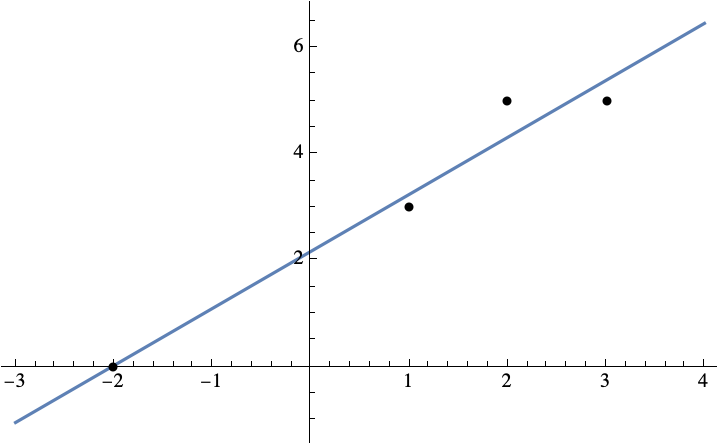
\includegraphics[width=8.5cm]{misc/linearregressionexample.png}
    \caption{Curve fitting example}
    \label{fig:curvefitting}
\end{figure}

One application (of many) of linear algebra, and specifically, the ability to find distances between different elements in any particular base is in \textit{curve fitting}. The process is a little abstract to describe generally, so first consider the following set of points (and corresponding graph, figure \ref{fig:curvefitting}):

$$(x,y) = (-2,0), (1,3), (2,5), (3,5)$$

It seems as if these points generally follow a linear trend, so we can try to find a line that fits the points as well as possible (\textit{note that a similar method to the following can be used for a polynomial trend, an exponential trend, etc, but with a little more work}). A line can be described by the equation $y = mx+b$, so our goal is to find the values of $m$ and $b$ that minimize the distance between the line and the points. We can write, for each individual point:

\begin{equation}
    \begin{split}
        y &= mx+b\\
        0 &= m(-2)+b\\
        3 &= m(1)+b\\
        5 &= m(2)+b\\
        5 &= m(3)+b
    \end{split}
\end{equation}

It should (hopefully) be clear that this is a system of equations for the variables $m$ and $b$. We can, as described earlier, consider this as a matrix equation of $A\vec{x} = \vec{y}$, where $A$ is the matrix of coefficients, $\vec{x}$ is the vector of variables, and $\vec{y}$ is the vector of $y$ values. We can write this as:

\begin{equation}
    \begin{split}
        \begin{bmatrix}
            0\\
            3\\
            5\\
            5
        \end{bmatrix} &= m \begin{bmatrix}
            -2\\
            1\\
            2\\
            3
        \end{bmatrix} + b \begin{bmatrix}
            1\\
            1\\
            1\\
            1
        \end{bmatrix}\\
        \begin{bmatrix}
            0\\
            3\\
            5\\
            5
        \end{bmatrix} &= \begin{bmatrix}
            m\\
            b\\
        \end{bmatrix} \begin{bmatrix}
            -2 & 1\\
            1 & 1\\
            2 & 1\\
            3 & 1
        \end{bmatrix}\\
        \vec{y} &= \vec{x}A
    \end{split}
\end{equation}

\textit{The last line here may seem a little bizarre, but should make more sense using the column-view of a matrix-vector multiplication.} We could solve this system of equations using Gaussian elimination as always, but it should be clear that it will be inconsistent. Intuitively, there is clearly no line that goes through all the points, and as such, there is no $m$ and $b$ that makes this equation true. You can also conclude this by looking at the rows of the $A$ matrix, which, if reduced, will not be consistent.

As such, we have to find the $m$ and $b$ that make this equation "as close to true" as possible. We define a new vector $\vec{z}$, where $\vec{z} = A\vec
x$. As described in an earlier section, we can find the shortest distance between two vectors by finding the projection of one onto the other, and we can then use this said projection to solve the system of equations. This is a fine method, but is very tedious and time-consuming, particularly for systems of multiple hundreds of data points.

For a non-linear trend (say, $y=ax^2+bx+c$), we can use the same method as above, but with a slightly different $A$ matrix, naturally.

% add figure here

\subsection{Orthogonality and the Transpose of a Vector}

Given a subspace $V$ of $\real^n$, we can define the \textit{orthogonal complement} of $V$ as the set of all vectors $\vec{u}$ such that $\vec{u}\cdot\vec{v} = 0$ for all $\vec{v}\in V$. This is denoted $V^\bot$. Finding this is fairly simple; for instance, take $V = \{\vec{v_1}, \vec{v_2}\}= \{\begin{bmatrix}-2\\
    2\\
    3\\
    0
\end{bmatrix}, \begin{bmatrix}-1\\
    1\\
    1\\
    1
\end{bmatrix}
\}$. To find $V^\bot$, we simply find the set of all vectors perpendicular to $\vec{v_1}$ \textbf{AND} $\vec{v_2}$. Let's define $\begin{bmatrix}
    x_1\\
    x_2\\
    x_3\\
    x_4\end{bmatrix} = \vec{x} \in V\bot$, so $\vec{v_1}\cdot\vec{x} = \vec{v_2}\cdot\vec{x} = 0$. Solving from here is fairly straightforward:

\begin{equation}
    \begin{split}
        -2x_1 + 2x_2 + 3x_3 +0x_4&= 0\\
        -x_1 + x_2 + x_3 +x_4 &= 0\\
    \end{split}
\end{equation}

\textbf{Notice:} this is the equivalent of multiplying the matrix $\begin{bmatrix}
    -2 & 2 & 3 & 0\\
    -1 & 1 & 1 & 1
\end{bmatrix}$ by $\vec{x}$. Since we are trying to find $\vec{x}$ when this product is $0$, we can see this instead as finding the kernel of this new matrix (ie ker($\begin{bmatrix}
    -2 & 2 & 3 & 0\\
    -1 & 1 & 1 & 1\end{bmatrix}$)).

Now, let us define $A$ as the matrix with columns equal to the vectors in $V$ (ie $A = \begin{bmatrix}\vec{v_1} \vec{v_2}\end{bmatrix}$). As previously discussed, the \textit{image} of a matrix is the span of its columns, so we can say that $im(A) = span(\vec{v_1}, \vec{v_2}) = V$.

To find how this work so far is useful, we need to introduce a new concept, namely the \textbf{transpose} of a matrix. Denoted, in our example, $A^T$, the transpose of a matrix is the matrix with rows equal to the columns of the original matrix:

\begin{equation}
    \begin{split}
        A^T &= \begin{bmatrix}
            -2&2&3&0\\
            -1&1&1&1
        \end{bmatrix}
    \end{split}
\end{equation}
    
\textbf{Please note that this is not the same as simply "flipping" the matrix on its side.} In actuality, you can think about this as the first element of the first row of $A$ becoming the first element of the first column of $A^T$, and so on.

Also notice that this matrix is equal to the matrix we found earlier when trying to find the perpendicular vectors to $\vec{v_1}$ and $\vec{v_2}$. So, continuing from our earlier logic, we can thus define the vectors perpendicular to $V$:

\begin{equation}
    \begin{split}
        \vec{x} &\in V^\bot\\
        \therefore \vec{x} &\in ker(\begin{bmatrix}
            -2 & 2 & 3 & 0\\
            -1 & 1 & 1 & 1\\
        \end{bmatrix}) = ker(A^T)\\
    \end{split}
\end{equation}

Putting all of this together, we can develop the following relationship between a matrix's transpose and orthogonal component:

\begin{equation}
    \begin{split}
        V^\bot &= ker(A^T)\\
        V &= im(A) \implies V^\bot = (im(A))^\bot\\
        &\therefore (im(A))^\bot = ker(A^T)\\
    \end{split}
\end{equation}

Working through the whole proof of this can be a little tedious, but it is very useful to understand. We can also slightly rewrite this conclusion to another useful form:

\begin{equation}
    \begin{split}
        (im(A))^\bot &= ker(A^T)\\
        ((im(A))^\bot)^{\red{\bot}} &= (ker(A^T))^{\red{\bot}}\\
        im(A) &= (ker(A^T))^\bot\\
        im(A^{\red{T}}) &= (ker(A^{T^{\red{T}}}))^{\bot}\\
        im(A^T) &= ker(A)^\bot
    \end{split}
\end{equation}

\subsection{Normal Equations}

While we showed a general form to use least squares to calculate the best fit line for an equation earlier, it would have resulted in having to find a projection, which, in higher dimensions, would prove unnecessarily tedious. Here, we build upon previous concepts to show a more efficient way.

Consider a set of data that, following the steps in section 3.1, we have defined as $A\vec{x} = \vec{b}$. Assuming this system is inconsistent (which would thus merit using least squares..), our goal is to find a vector $\vec{y}$ that is as close to $\vec{b}$ as possible. We know we can do this using projections, and thus write:

\begin{equation}
    \begin{split}
        A\vec{x} = \vec{y} = proj_{im(A)}(\vec{b})
    \end{split}
\end{equation}

We can more thoroughly define $\vec{b}$ as well. $\vec{b}$ can be thought of as being the sum of $\vec{y}$ in one direction, and some other vector perpendicular to $\vec{y}$. We've established that $\vec{y} \in im(A)$, so this perpendicular vector is in $A^\bot$. Even more specifically, we can write:

\begin{equation}
    \begin{split}
       \vec{b} &= proj_{im(A)}(\vec{b}) + proj_{im(A)^\bot}(\vec{b})\\
       proj_{im(A)}(\vec{b}) &= \vec{b} - proj_{im(A)^\bot}(\vec{b})\\
    \end{split}
\end{equation}

Substituting into equation 25, and doing some (admittedly unintuitive) algebra:

\begin{equation}
    \begin{split}
        A\vec{x} &= \vec{b} - proj_{im(A)^\bot}(\vec{b})\\
        \red{A^T}(A\vec{x}) &= \red{A^T}(\vec{b} - proj_{im(A)^\bot}(\vec{b}))\\
        A^T A \vec{x} &= A^{T} \vec{b} - A^{T} proj_{im(A)^\bot}(\vec{b})\\
    \end{split}
\end{equation}

Recall that $(im(A))^\bot = ker(A^T)$, so we can write:

\begin{equation}
    \begin{split}
        A^T A \vec{x} &= A^{T} \vec{b} - A^{T} proj_{im(A)^\bot}(\vec{b})\\
        A^T A \vec{x} &= A^{T} \vec{b} - A^{T} proj_{\red{ker(A^T)}}(\vec{b})
    \end{split}
\end{equation}

However, in this final line, $\vec{b}$ is being projected onto the kernel of $A^T$, resulting in a vector in the kernel of $A^T$, which, when then multiplied by $A^T$ itself, simply results in $\vec{0}$. Thus, we can write our final form:

\begin{equation}
    \begin{split}
        A^T A \vec{x} &= A^{T} \vec{b}\\
    \end{split}
\end{equation}

In all, the goal is to find $\vec{x}$, which now only requires a couple of matrix operations, rather than a whole mess of projections. This equation is known as the \textbf{normal equation}.

\subsection{The Determinant}

The \textbf{determinant} of a matrix is a scalar value that can be used to describe many properties of a matrix, denoted either as $det(A)$ or $|A|$. In particular, it can be used to describe whether a matrix is invertible without needing to actually invert it; by extension, a determinant only exists for a square matrix. The formula for the determinant of a $2x2$ matrix can be derived through trying to invert it (by augmenting it with the identity matrix):

\begin{equation}
    \begin{split}
        \begin{array}[t][{@{}cc|cc@{}}]
            a & b & 1 & 0 \\
            c & d & 0 & 1 \\
        \end{array}\\
        ...\\
        \begin{array}[t][{@{}cc|cc@{}}]
            1 & \frac{b}{a} & \frac{1}{a} & 0 \\
            0 & \red{d-\frac{bc}{a}} & -\frac{1}{a} & 1 \\
        \end{array}\\
    \end{split}
\end{equation}

Without even finishing the elimination, it should be clear that the term $d-\frac{bc}{a}$ (in red) cannot equal 0 in order for the matrix to be invertible. We can rewrite this term as $ad-bc$; this is the determinant of a $2x2$ matrix. 

\subsubsection{Determinants of Larger Matrices}

The determinant of matrices larger than 2x2 could be derived similarly, but the work is tedious. Instead, you can break down the matrix into smaller matrices, and use the determinant of the smaller matrices to find the determinant of the larger matrix. For example, consider the following $3x3$ matrix, $A = \begin{bmatrix}
    a & b & c\\
    d & e & f\\
    g & h & i
\end{bmatrix}$. 

To solve for the determinant of $A$, we can pick any particular row or column, and break the matrix into smaller matrices based on it. For example, we can pick the first row, and break the matrix into $2x2$ matrices:

\begin{equation}
    \begin{split}
        det(A) = a*det(\begin{bmatrix}
            e & f\\
            h & i
            \end{bmatrix}) - b*det(\begin{bmatrix}
            d & f\\
            g & i
            \end{bmatrix}) + c*det(\begin{bmatrix}
            d & e\\
            g & h
            \end{bmatrix})
    \end{split}
\end{equation}

Note that each "submatrix" used in this case is the matrix of $A$ without the respective row or column that the coefficient of our row in question is in. Also note that we multiplied the second term by $-1$. In general, we have to multiply by the corresponding sign in a "sign matrix", in which the top left corner is positive, and the sign alternates from there.

We can finish solving this using our determinant formula of 2x2 matrices:

\[
    det(A) = a(ei - fh) - b(di-fg) + c(dh-eg)
\]

Theoretically, you could use this formula as a general formula for any 3x3 matrix, but, in practice, it is far easier to simply use the algorithm described above for the particular case.

For determinants of higher order matrices, the same general formula applies, but the resulting "submatrices" have to then be broken down more.

\subsubsection{Properties of Determinants}

It is helpful to remember a few properties of determinants of different matrices to make certain problems easier. For matrices $A$ and $B$:

\begin{itemize}
    \item $det(A) = det(A^T)$
    \item $det(A) = -det(A)$, if a row of $A$ is exchanged
    \item $det(kA) = k^n det(A)$, where $n$ is the order of $A$
    \item $det(AB) = det(A)det(B)$
    \item $det(A) + det(B) \neq det(A+B)$
\end{itemize}

\subsection{Applications to Area and Volume}

\subsubsection{Area}

Take a parallelogram who's sides are defined by the length of vectors $\vec{v} = \begin{bmatrix}
    a\\
    b
\end{bmatrix}$ and $\vec{u} = \begin{bmatrix}
    c\\
    d
\end{bmatrix}$. You can also think of this as the base being defined as $\vec{v}$, then being translated upwards by $\vec{u}$; see figure \ref{fig:parallelogram}.

\begin{figure}
    \centering
    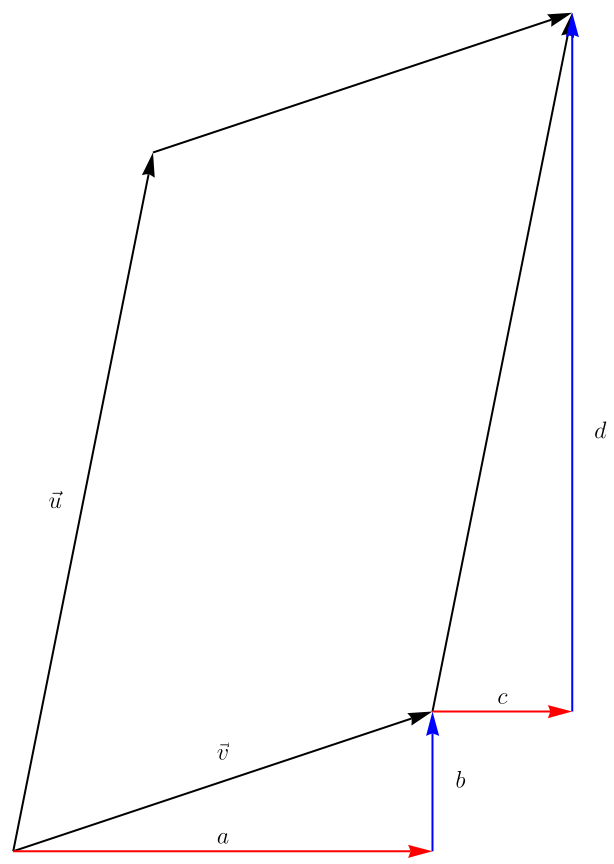
\includegraphics[width=5cm]{misc/parallelogram.png}
    \caption{A parallelogram defined by vectors $\vec{v}$ and $\vec{u}$}
    \label{fig:parallelogram}
\end{figure}

We can see this image as the area of a rectangle removed by the area of 2 triangles on either side of the parallelogram:

\begin{equation}
    \begin{split}
    A &= (a+b)(c+d) - 2 (\frac{1}{2}(c(a+b))) + 2(\frac{1}{2}(b(c+d)))\\
    A &= (a+b)(c+d) - ca - cb - bc - bd\\
    A &= ac + ad + bc + bd - ca - bc - bc - bd\\
    &= ad - bc = |\begin{bmatrix}
        a & b\\
        c & d
        \end{bmatrix}|
    \end{split}
\end{equation}

Note that this is simply the determinant of the matrix defined by the vectors $\vec{v}$ and $\vec{u}$ (though you may have to take the absolute value, depending on the context).

\subsubsection{Volume}

Consider a parallelepiped, whose sides are defined by the vectors $\vec{v} = \begin{bmatrix}
    a\\
    b\\
    c
\end{bmatrix}$, $\vec{u} = \begin{bmatrix}
    d\\
    e\\
    f
\end{bmatrix}$, and $\vec{w} = \begin{bmatrix}
    g\\
    h\\
    i
\end{bmatrix}$.

The volume of such a figure can be found with:

\[
    A = \vec{u} \cdot (\vec{v}\times \vec{w})
    \]

To derive this expression, first consider the base, defined by the vectors $\vec{v}$ and $\vec{w}$. The area of this base is the height times the matrix, which, with a little trigonometry, can be shown to equal $||\vec{v}||||\vec{w}||\sin \theta$, with $\theta$ representing the angle between the two vectors. This, as a matter of fact, is simply another way to define cross product of $\vec{v}$ and $\vec{w}$, namely $\vec{v}\times\vec{w} = A_{base}$.

Now, to find the volume we next need the height. We can find this by picturing a right triangle with a hypotenuse defined by $\vec{u}$, and the height in question actually being a scalar multiple of the cross product of $\vec{v}$ and $\vec{w}$. With a little more trigonometry, it is clear that this value is simply equal to $||\vec{u}||\cos \alpha$, with $\alpha$ representing the angle between $\vec{u}$ and $\vec{v}$. 

Multiplying the height by the area of the base, we get the volume of the parallelepiped:

\begin{align*}
A = ||\vec{u}||\cos\alpha * (\vec{v} \times \vec{w})\\
= \vec{u}\cdot(\vec{v} \times \vec{w})\\
\end{align*}

\subsection{Adjugates}

To define adjugates of a matrix, the idea of a \textit{cofactor} must first be defined. The cofactor of a matrix is the matrix of the determinants of a matrix's submatrices, with the signs of the submatrices alternating. For example, take $A = \begin{bmatrix}
    a & b\\
    c & d
\end{bmatrix}$. The cofactors of $A$ can be found as follows (\textit{note the similarity between the work here and the method used to find the determinant of a large matrix}):

\begin{align*}
    c_{1,1} = det(\begin{bmatrix}
        d
    \end{bmatrix}) = d\\
    c_{1,2} = det(\begin{bmatrix}
        c
    \end{bmatrix}) = -c\\
    c_{2,1} = det(\begin{bmatrix}
        b
    \end{bmatrix}) = -b\\
    c_{2,2} = det(\begin{bmatrix}
        a
    \end{bmatrix}) = a\\
    \begin{bmatrix}
        c_{1,1} & c_{1,2}\\
        c_{2,1} & c_{2,2}
    \end{bmatrix} = \begin{bmatrix}
        d & -c\\
        -b & a
    \end{bmatrix}
\end{align*}

Notice the similarity between this and the formula for computing the inverse of $A$:

\begin{equation}
    \begin{split}
    A^{-1} &= \frac{1}{det(A)}\begin{bmatrix}
       d & -b\\
        -c & a
    \end{bmatrix}\\
    \end{split}
\end{equation}

The matrix of cofactors we derived is simply the transpose of the matrix in this equation, which is called the \textbf{adjugate} of $A$, denoted adj$(A)$. We can thus say the following:

\begin{equation}
    \begin{split}
    A^{-1} &= \frac{1}{det(A)}adj(A)\\
    \end{split}
\end{equation}

Note that this formula is, clearly, undefined if $det(A) = 0$; this should make sense, since, by definition of the determinant, the determinant of a matrix is 0 if and only if the matrix is singular.

We can also prove this formula for the general case of an $n \times n$ matrix (for those interested...).

\renewcommand{\qedsymbol}{$\blacksquare$}

\begin{proof}
    Consider the inverse matrix $A^{-1}$, with columns $\vec{x_1}, \vec{x_2}, \dots, \vec{x_n}$, ie \[A^{-1} = 
    \begin{bmatrix} 
        | & | & &|\\
        \vec{x_1} & \vec{x_2} & \dots & \vec{x_n}\\
        | & | & &|
    \end{bmatrix}\] We can describe the $j$th row of $A^{-1}$ by $\vec{x_j} = A^{-1}\vec{e_j}$, which we can rewrite $A\vec{x_j}= A(A^{-1}\vec{e_j}) = I_n \vec{e_j} = \vec{e_j}$. Using Cramer's Rule (explained below), we can find the $i$th entry of $\vec{x_j}$: \[x_{i,j} = \frac{det(A_i)}{det(A)}\] where $A_i$ is the matrix $A$ with the $i$th column replaced by $\vec{e_j}$. Finding the determinant of $A_i$ by expanding upon the $i$th row, we see that $det(A_i)$ is simply the $i$th entry of the cofactor matrix of $A$, ie $det(A_i) = c_{i,j}$. Thus, \[x_{i,j} = \frac{c_{i,j}}{det(A)}\] We can now write the $j$th column of $A^{-1}$ as \[\vec{x_j} = \frac{1}{det(A)}\begin{bmatrix}
        c_{1,j}\\
        c_{2,j}\\
        \vdots\\
        c_{n,j}
    \end{bmatrix}\] which is simply the $j$th column of the adjugate matrix of $A$, adj$(A)$. Thus, we can say that \[A^{-1} = \begin{bmatrix} 
        | & | & & |\\
        \vec{x_1} & \vec{x_2} & \dots & \vec{x_n}\\
        | & | & & |
    \end{bmatrix} = \frac{1}{det(A)}adj(A)\]
\end{proof}

Also note that we can rewrite this expression as:

\begin{equation}
    \begin{split}
        \red{A*det(A)}A^{-1} &= \red{A*det(A)}\frac{1}{det(A)} adj(A)\\
        det(A) &= A * adj(A)\\
    \end{split}
\end{equation}

\subsection{Cramer's Rule}

Explained \hyperref{http://notes.louismeunier.net/Calculus%20A,%20B/calculus.pdf#page=56}{}{}{here.}

In summary: we can find the solution of the $i$th variable (ie, $x_i$) in a system of $n$ equations of $n$ variables of the form $a x_1 + b x_2 + ... + z x_n = c$ with the formula:

\begin{equation}
    \begin{split}
        x_i &= \frac{det(A_i)}{det(A)}\\
    \end{split}
\end{equation}

Where $A$ is the matrix of coefficients, and $A_i$ is the matrix of coefficients with the $i$th column replaced by the vector of solutions of the respective equations.

\subsection{Linear Discrete Dynamical Systems}

Breaking down the definition of a linear discrete dynamical system:

\begin{itemize}
    \item \textit{linear:} output of the system is a linear combination of the inputs (recall linear transformations) 
    \item \textit{discrete:} the system is defined only for a finite number of inputs (ie, integers, $\integers$)
    \item \textit{dynamical:} the vectors in the system change with time
\end{itemize}

These types of systems are often used to describe changes in several populations which depend on one another (whether inversely or directly).

For example, consider a system of two populations, $x$ and $y$, where $x$ is a predator of $y$. Say we can model the change in each population as follows:

\begin{equation}
    \begin{cases}
      x(t+1) = 0.5x(t) + 0.2y(t)\\
      y(t+1) = -0.3x(t) + 1.5y(t)\\
    \end{cases} 
\end{equation}

We can interpret this system as follows:

\begin{itemize}
    \item The population of $x$ in a particular year ($t+1$) depends on its population in the previous year ($t$) and the population of $y$ in the previous year ($t$); in particular, the population of $x$ decreases by 50\% and increases by 20\% for each $y$ in the previous year.
    \item The population of $y$ in a particular year ($t+1$) depends on its population in the previous year ($t$) and the population of $x$ in the previous year ($t$); in particular, the population of $y$ decreases by 30\% and increases by 150\% for each $y$ in the previous year.
\end{itemize}

This changes in population could be due to predation (clearly, as $x$ is a predator of $y$), reproduction/survival rates, or any other factor.

This system can be represented as a matrix times a vector; specifically, a matrix of the coefficients of the system, and a vector of the populations in the previous year. If we define $\vec{P}(t)$ as the population vector in year $t+1$, we can write the system as:

\begin{equation}
    \begin{split}
        \vec{P}(t+1) = \begin{bmatrix}
            x(t+1)\\
            y(t+1)
        \end{bmatrix} = \begin{bmatrix}
            0.5 & 0.2\\
            -0.3 & 1.5
        \end{bmatrix}\begin{bmatrix}
            x(t)\\
            y(t)
        \end{bmatrix} = A\vec{P}(t)\\
    \end{split}
\end{equation}

\textit{This matrix is often called a \textbf{Leslie matrix}, when used in population dynamics.}

This form of equation, while helpful when $P(t)$ is known for a particular $t$, but does not make it clear how $P$ changes over time. However, seeing as how this equation is recursively defined, we can say the following: 

\begin{equation}\label{eqn:poft}
    \begin{split}
        \vec{P}(t) &= A\vec{P}(t-1)\\
        &= A(A\vec{P}(t-2))\\
        &= A^2\vec{P}(t-2)\\
        &= A^3\vec{P}(t-3)\\
        &= \dots\\
        &= A^t\vec{P}(0)\\
    \end{split}
\end{equation}

This has somewhat generalized our equation, but we still need the initial population in order to find the population at any given time. The following section will show how we can modify this equation accordingly...

\subsection{Eigenstuff}
\subsubsection{Application to Linear Discrete Dynamical Systems}
An \textbf{eigenvector} of a matrix $A$ is a vector $\vec{v} \neq \vec{0}$ such that $A\vec{v} = \lambda\vec{v}$, where $\lambda$ is a scalar. In other words, the eigenvector is a vector that is simply scaled by some scalar $\lambda$ when multiplied by the matrix $A$. This scalar is the corresponding \textbf{eigenvalue} of the eigenvector.

Reconsider the previous section, where we said that $\vec{P}(t) = A^t \vec{P}(0)$. Lets say we are given two linearly independent eigenvectors of $A$ \textit{(which, as we'll say later, is the max number of eigenvectors $A$ can have since it is 2x2)}, $\vec{v_1}$ and $\vec{v_2}$, and their corresponding eigenvalues $\lambda_1$ and $\lambda_2$. WE know that:
\begin{align*}
        A\vec{v_1} &= \lambda_1\vec{v_1}\\
        A\vec{v_2} &= \lambda_2\vec{v_2}\
\end{align*}
We can multiply each of these by $A$ again ($t$ times...):
\begin{align*}
    \red{A}A\vec{v_1} &= \red{A}\lambda_1\vec{v_1}\\
    A^2 \vec{v_1} &= \lambda_1A\vec{v_1}\\
    &= \lambda_1^2\vec{v_1}\\
    &\cdots\\
    A^t \vec{v_1} &= \lambda_1^t\vec{v_1}; \text{similarly: } A^t \vec{v_2} = \lambda_2^t\vec{v_2}
\end{align*}
Let's say we are given $\vec{P}(t_0) = \begin{bmatrix}
    a\\
    b\end{bmatrix}$ for some time; we can consider this as the initial population, $\vec{P}(0)$, and write:
\begin{align*}
    \vec{P}(t) = A^t\vec{P}(0) &= A^t\begin{bmatrix}
        a\\
        b\end{bmatrix}\\
\end{align*}
Since $\vec{v_1}, \vec{v_2}$ are two linearly independent vectors (which is generally true of eigenvectors, but will be explained more later...) in $\real^2$, we can therefore say:
\begin{align*}
    \begin{bmatrix}
        a\\
        b\end{bmatrix} &= c_1\vec{v_1} + c_2\vec{v_2}; c_1, c_2 \in \real
\end{align*}
Substituting this into the previous equation for $\vec{P}(0)$, we get:
\begin{align*}
    \vec{P}(t) = A^t(c_1\vec{v_1} + c_2\vec{v_2})
\end{align*}
We can distribute the $A^t$:
\begin{align*}
    \vec{P}(t) &= c_1A^t\vec{v_1} + c_2A^t\vec{v_2}
\end{align*}
However, since $\vec{v_1}, \vec{v_2}$ are eigenvectors of $A$, we established that $A^t\vec{v_1} = \lambda_1^t\vec{v_1}$ and $A^t\vec{v_2} = \lambda_2^t\vec{v_2}$, so we can substitute these into the previous equation:
\begin{align*}
    \vec{P}(t) &= c_1\lambda_1^t\vec{v_1} + c_2\lambda_2^t\vec{v_2}
\end{align*}
This is a far more usable form of the equation, since, if we can find the eigenvalues and eigenvectors of $A$, we can find the population at any given time, given the population at some time and the corresponding matrix $A$. This form of equation is called the \textbf{closed-form} for $\vec{P}(t)$.

\subsubsection{Computing Eigenvalues, Eigenvectors}

Recall how we defined an eigenvector $\vec{v}$ of a matrix $A$:
\begin{align*}
    A\vec{v} = \lambda \vec{v}
\end{align*}
Moving all the terms to the same side, we get:
\begin{align*}
    \lambda \vec{v} - A\vec{v}&= \vec{0}\\
    \vec{v}(\lambda - A) &= \vec{0}
\end{align*}
This, however, is not currently possible to solve: $A$ is a matrix and $\lambda$ is a constant, so we cannot subtract one from the other. However, we can multiply both sides of the equation by $I$, which will leave $A$ the same (and $0$, of course):
\begin{align*}
    \red{I}*\vec{v}(\lambda - A) &= \vec{0}*\red{I}\\
    \vec{v}(\lambda I - A) &= \vec{0}
\end{align*}
Notice that $\lambda I - A$ is a matrix itself now. Since $\vec{v}$ multiplied by this new matrix is equal to $\vec{0}$, then $\vec{v}$ must be in the kernel of $\lambda I - A$. As such, in order for $\vec{v}$ to even have a kernel, then $\lambda I - A$ must be singular (not invertible), and by extension, its determinant must equal $0$. Therefore, we can write:
\begin{align*}
    \det(\lambda I - A) &= 0
\end{align*}

Solving this formula typically results in a polynomial in terms of $\lambda$ equal to 0; this is called the \textbf{characteristic polynomial} (denoted $c_A(\lambda)$) of $A$. The roots of this polynomial are the eigenvalues of $A$. Plugging these values into the original equation for $\vec{v}$, we can find each corresponding eigenvector of $A$.

Taking the example from the previous section, we can find the eigenvalues and eigenvectors of $A = \begin{bmatrix}
    0.5 & 0.2\\
    -0.3 & 1.5\\
\end{bmatrix}$ as follows (\textit{using our formula for the determinant of a 2x2 matrix}):
\begin{align*}
    0 = det(\lambda I - A) &= det(\lambda I - \begin{bmatrix}
        0.5 & 0.2\\
        -0.3 & 1.5\\
    \end{bmatrix})\\
    &= det(\begin{bmatrix}
    \lambda-0.5 & -0.2\\
    0.3 & \lambda-1.5\\
    \end{bmatrix})\\
    &= (\lambda - 0.5)(\lambda - 1.5) - 0.3(-0.2)\\
    &= \lambda^2-2\lambda+0.81\\
    &\dots\\
    & \lambda = 0.564, 1.436
\end{align*}

We could then plug these values into the original formula to find the corresponding eigenvectors.

\subsubsection{Algebraic Multiplicity}

Recall the characteristic polynomial of matrix $A$, $c_A(\lambda) = |\lambda I - A|$. Sometimes, this polynomial will have multiple of the same roots, ie, multiple of the same eigenvalue; this will arise if the polynomial is, say, in the form $(\lambda_1-a)^n$ where $n\geq 2$. When this occurs, we can say that this particular eigenvalue has \textbf{algebraic multiplicity} $n$.

\subsubsection{Eigenspaces and Bases}

An \textbf{eigenspace} is the set of vectors that are eigenvectors of a matrix $A$ with a particular eigenvalue $\lambda$, denoted $E_{\lambda}$. 

For instance, take the matrix $A = \begin{bmatrix}
    1 & 1\\
    0 & 1\\
\end{bmatrix}$. Solving for the eigenvalues:

\begin{align*}
    0 &= |\lambda I - A|\\
    &= |\begin{bmatrix}
        \lambda-1 & -1\\
        0 & \lambda-1\\
    \end{bmatrix}|\\
    &= (\lambda-1)^2 = 0\\
    &\lambda = 1\\
\end{align*}

\textit{Note that the eigenvalue of this matrix has algebraic multiplicity $2$.} Finding the corresponding eigenvector(s?):

\begin{align*}
    ker(\lambda I - A) &= ker(\begin{bmatrix}
        \lambda - 1 & -1\\
        0 & \lambda-1\\
    \end{bmatrix})\\
    &= ker(\begin{bmatrix}
        0 & -1\\
        0 & 0\\
    \end{bmatrix})\\
    &= \{\begin{bmatrix}
        x\\
        y
    \end{bmatrix} = \begin{bmatrix}
        t\\
        0
    \end{bmatrix}, t \in \real \}
\end{align*}

As such, we can say that the eigenspace of $A$ with eigenvalue $\lambda = 1$ is this same set, ie, $E_1=span(\begin{bmatrix}
    1\\
    0\end{bmatrix})$. In other words, the eigenspace for a matrix $A$'s particular eigenvalue $\lambda$ has an eigenspace $E_\lambda = ker(\lambda I - A)$.

Note that, in this situation, there exists only one eigenvector, and as such, it is impossible to span $R^2$ (which this matrix is in) with only eigenvectors. If this were possible, however, then we would have found a \textbf{eigenbasis} for $R^2$, as the eigenvectors would span the entire space. This is what happened in the earlier example: the eigenvectors spanned the entire space, and as such, we found an eigenbasis, and were able to solve the discrete dynamical system by rewriting the equation in terms of the eigenvectors. It is not possible to use the same method if an eigenbasis does not exist.

Another relevant term to know is the \textbf{geometric multiplicity} of a particular eigenvalue, which corresponds to the dimension of its eigenspace (ie, $dim(ker(\lambda I - A))$). In this example, the geometric multiplicity of $\lambda = 1$ is $1$, as the eigenspace is a line. Also note the following inequality (which is too difficult to prove in this course):

\begin{equation}
    1 \leq \text{geom. multiplicity of } \lambda_i \leq \text{alg. multiplicity of } \lambda_i
\end{equation}

% add more about multiplicity and stuff

\subsection{Diagonalization}

A diagonalized matrix $A$ (such that $T(\vec{x}) = A\vec{x}$) is one that can be written as $[T(\vec{x})]_{\mathfrak{B}} = B[\vec{x}]_{\mathfrak{B}}$ where $B$ has the form $\begin{bmatrix}
    \lambda_1 & 0 & \dots & 0\\
    0 & \lambda_2 & \dots & 0\\
    \vdots & \vdots & \ddots & \vdots\\
    0 & 0 & \dots & \lambda_n
\end{bmatrix}$, where $\lambda_1, \lambda_2, \dots, \lambda_n$ are the eigenvalues of $A$. By extension, \textbf{a matrix is diagonalizable if and only if it has a eigenbasis.} Since a matrix can only have an eigenbasis if each of its eigenvectors has an algebraic multiplicity of 1, we can say that a matrix is diagonalizable if and only if each of its eigenvalues has algebraic multiplicity of 1 (note that there are many other ways to state this same property...).

For instance, take some matrix $A$, with eigenvalues $\lambda_1 = 3$, $\lambda_2 = 2$, and $\lambda_3 = -2$, and corresponding eigenvectors $\vec{v_1} = \begin{bmatrix}
    -3\\
    1\\
    0\end{bmatrix}$, $\vec{v_2}=\begin{bmatrix}
    1\\
    0\\
    5\end{bmatrix}$, and $\vec{v_3}=\begin{bmatrix}
    0\\
    2\\
    7\end{bmatrix}$, respectively. We can take $\mathfrak{B} = \{\vec{v_1}, \vec{v_2}, \vec{v_3}\}$, a basis of $R^3$ spanned by the eigenvectors. We can then solve for the $B$ matrix of this situation:

\begin{align*}
    T(\vec{x}) &= A\vec{x}\\
    T(\vec{v_1}) = A * \vec{v_1} &= \lambda_1\vec{v_1} = 3 \vec{v_1}\\
    T(\vec{v_2}) = A * \vec{v_2} &= \lambda_2\vec{v_2} = 2 \vec{v_2}\\
    T(\vec{v_3}) = A * \vec{v_3} &= \lambda_3\vec{v_3} = -2 \vec{v_3}\\
    \therefore B &= \begin{bmatrix}
        [T(\vec{v_1})]_{\mathfrak{B}}, [T(\vec{v_2})]_{\mathfrak{B}}, [T(\vec{v_2})]_{\mathfrak{B}}
    \end{bmatrix}\\
    &= \begin{bmatrix}
        3 & 0 & 0\\
        0 & 2 & 0\\
        0 & 0 & -2
    \end{bmatrix}
\end{align*}

Note that this matrix $B$ has the eigenvalues of $A$ on its diagonal, and thus, is diagonalizable.

To phrase this in a more general sense, a matrix $A$ is diagonalizable if you can write $A = SBS^{-1}$, where $S$ is an invertible matrix and $B$ is a diagonal matrix. In this form, we can rewrite $A^n$ in a closed form as follows:

\begin{align*}
    A^n &= (SBS^{-1})^n\\
    &= SBS^{-1}SBS^{-1} \dots SBS^{-1}\\
    &= SB^{n}S^{-1}\\
\end{align*}

This form is far easier to compute than computing $n$ products of $A$, since $B^n$, being a diagonal matrix, is simply:

\begin{align*}
    B^n &= \begin{bmatrix}
        \lambda_1 & 0 & \dots & 0\\
        0 & \lambda_2 & \dots & 0\\
        \vdots & \vdots & \ddots & 0 \\
        0 & 0 & 0 & \lambda_n
    \end{bmatrix}^n\\
    &= \begin{bmatrix}
        \lambda_1^n & 0 & \dots & 0\\
        0 & \lambda_2^n & \dots & 0\\
        \vdots & \vdots & \ddots & 0 \\
        0 & 0 & 0 & \lambda_n^n
    \end{bmatrix}
\end{align*}

\textit{Note that, since we've written $A^n = SB^nS^{-1}$, we can say that $A^n$ is diagonalizable if $A$ is diagonalizable. It also has the same eigenvectors as $A$, since $S$ does not change, and it has the same eigenvalues as $A$ but raised to the power of $n$.}

In the context of a linear discrete dynamical system, where $\vec{x}(t) = A^t\vec{x}(0)$, we can derive the general closed form expression in a different way. We want $\vec{x}(0) = c_1\vec{v_1} + \dots + c_n\vec{v_n}$, where $\vec{v_1}, \vec{v_2}, \dots, \vec{v_n}$ are the eigenvectors of $A$. As such, we can say $\vec{x}(0) = S\begin{bmatrix}
    c_1\\
    c_2\\
    c_n
\end{bmatrix}_{\mathfrak{B}}$, where $\mathfrak{B} = \{\vec{v_1}, \vec{v_2}, \dots, \vec{v_n}\}$. We can then say:

\begin{align*}
    \vec{x}(t) &= A^t\vec{x}(0)\\
    &= (SBS^{-1})^t\vec{x}(0)\\
    &= \begin{bmatrix}
        \vec{v_1} & \dots & \vec{v_n}
    \end{bmatrix}\begin{bmatrix}
        \lambda_1^t & & \\
        & \ddots & \\
        & & \lambda_n^t
    \end{bmatrix}S^{-1} \vec{x}(0)\\
    &= \begin{bmatrix}
        \vec{v_1} & \dots & \vec{v_n}
    \end{bmatrix}\begin{bmatrix}
        \lambda_1^t & & \\
        & \ddots & \\
        & & \lambda_n^t
    \end{bmatrix}S^{-1}S\begin{bmatrix}
        c_1\\
        \vdots\\
        c_n
    \end{bmatrix}\\
    &= \begin{bmatrix}
        \vec{v_1} & \dots & \vec{v_n}
    \end{bmatrix}\begin{bmatrix}
       c_1 \lambda_1^t & & \\
        & \ddots & \\
        & & c_n\lambda_n^t
    \end{bmatrix}\\
    &= c_1 \lambda_1^t\vec{v_1} + \dots + c_n\lambda_n^t\vec{v_n}\\
\end{align*}

This is the same form as derived before for $\vec{x}(t)$.

\subsubsection{Properties of Diagonalizable Matrices}

\begin{itemize}
    \item If $A$ is diagonalizable, so is $A^n$ for any $n \in \mathbb{N}$. $A^n$ also has the same eigenvectors as $A$ and the same eigenvalues as $A$ but raised to the power of $n$.
    \item If $A$ is diagonalizable and invertible, then $A^{-1}$ is also diagonalizable. Proof:
    
    \begin{align*}
        A &= SDS^{-1}\\
        A^{\red{-1}} &= (SDS^{-1})^{\red{-1}}\\
        &= S^{-1}D^{-1}S\\
    \end{align*}

    Thus, we can write $A^{-1}$ in the form required for it to be diagonalizable. We can also see that $A^{-1}$ has the same eigenvalues as $A$ but raised to the power of $-1$.
    \item If $A$ and $B$ are diagonalizable matrices of the same dimension, \textbf{their sum is not necessarily} diagonalizable. Counterexample:

    \begin{align*}
        A = \begin{bmatrix}
            1 & 1\\
            0 & 2
        \end{bmatrix}, &\quad B = \begin{bmatrix}
            -1 & 0\\
            0 & -2
        \end{bmatrix}\\
        A + B &= \begin{bmatrix}
            0 & 1\\
            0 & 0
        \end{bmatrix} (\neq SBS^{-1})\\
    \end{align*}
    \item If $A$ and $B$ are diagonalizable matrices of the same dimension, \textbf{their product is not necessarily} diagonalizable. Counterexample:
    
    \begin{align*}
        \begin{bmatrix}
            1 & 0\\
            0 & -1
        \end{bmatrix}\begin{bmatrix}
            1 & 1\\
            0 & -1
        \end{bmatrix} &= \begin{bmatrix}
            1 & 1\\
            0 & 1
        \end{bmatrix} (\neq SBS^{-1})\\
    \end{align*}
\end{itemize}

\subsection{Extensions of Eigenvalues, etc}

Take a general 2x2 matrix $A = \begin{bmatrix}
    a & b\\
    c & d
\end{bmatrix}$. Solving for the eigenvalues of $A$:

\begin{align*}
    0 = |\lambda I - A| &= |\begin{bmatrix}
        \lambda - a & -b\\
        -c & \lambda - d
    \end{bmatrix}|\\
    &= \lambda^2 - (\red{a+d})\lambda + (\red{ad - bc})\\
\end{align*}

Note that the constant value of the characteristic polynomial of $A$ is simply the determinant of $A$, $\red{ad - bc}$.

The term in from of $\lambda$, $\red{a+d}$, is the sum of the main diagonal of $A$ which is known as the \textbf{trace} of $A$ (denoted $tr(A)$). 

Now, say that the eigenvalues of $A$ are $\alpha$ and $\beta$; thus, the $C_A(\lambda)$ can also be written:

\begin{align*}
    (\lambda - \alpha)(\lambda - \beta) &= 0\\
    \lambda^2 - (\red{\alpha + \beta})\lambda + \red{\alpha\beta} &= 0
\end{align*}
    
Thus, we can write that $a+d = \alpha + \beta$ and $ad - bc = \alpha\beta$, and thus, the trace of a matrix is the sum of its eigenvalues, and its determinant is the product of its eigenvalues. 

This pattern also applies to higher order matrices (but won't be proven here...). In summary, for a matrix $A$ of dimension $n$:

\begin{align*}
    tr(A) &= \sum_i^n \lambda_i \\
    det(A) &= \prod_i^n \lambda_i
\end{align*}

Note that eigenvalues of multiplicity $\geq 2$, the eigenvalues must included that many times in the sum/product.

\subsection{More on Dynamical Systems}

\subsubsection{Stability}

\textbf{Definition: } a dynamical system $\vec{x}(t+1) = A\vec{x}(t)$ is considered \textit{stable} if $A$ is a diagonalizable matrix and all solutions $\vec{x}(t)$ approach $\vec{0}$ as $t \to \infty$, regardless of the initial $\vec{x}{0}$. 

Take a system defined as $\vec{x}(t) = c_1 (\frac{1}{2})^t \begin{bmatrix}
    3\\
    -1
\end{bmatrix} + c_2 (\frac{1}{4})^t \begin{bmatrix}
    0\\
    1
\end{bmatrix}$, where $\vec{x}(0) = c_1\begin{bmatrix}
    3\\
    -1
\end{bmatrix} + c_2\begin{bmatrix}
    0\\
    1
\end{bmatrix}$. Intuitively, it should be clear that as $t \to \infty$, $\vec{x}(t)$ approaches $\vec{0}$, since for both $(\frac{1}{2})^t$ and $(\frac{1}{4})^t$, as $t$ increases, vectors they are being multiplied to approach $\vec{0}$. We can thus say that a linear dynamical system is stable if the eigenvalues of $A$ are all less than $1$ in magnitude (ie $|\lambda_i| < 1$). Since the eigenvalues do not depend on the initial condition of the system, we can say that the system is stable.

Consider also the \textbf{phase portrait} of this system. A phase portrait is a graph of the system's solutions over time, which essentially treats $\vec{x}(t)$ as a parametric plot of the $x$ and $y$ coordinates of the vector. The phase portrait of the system is shown below:

\newpage
\section{Summary of Terms}

This course relies \textbf{heavily} on vocabulary. Below is a brief conglomeration (ignore the oxymoron) of these terms.

\subsection{Notation}
    \begin{itemize}
        \item $\real$: real numbers
        \item $\integers$: integers
        \item $\naturals$: natural numbers
        \item $\real^n$: the $n$th real dimension
        \item $\{...\}$: set
        \item $\in$: "is in"
        \item $\exists$: "exists"
        \item $\therefore$: "therefore"
        \item $\Vec{u}$: vector named "$u$"
        \item $\Vec{0}$: "0 vector", vector of any dimension with all $0$'s
        \item $\vec{e}_i$: "unit vector", vector of any dimension with all $0$'s except for the $i$th element, which is $1$
        \item $f: A \to B$: "a function $f$ takes inputs of dimension $A$ and returns outputs of dimensions $B$"
        \item $T \circ S$: "$T$ composed with $S$"
        \item $\mathfrak{B}, \mathfrak{C}, ...$: a basis of some $\real^n$
        \item $[\vec{x}]_{\mathfrak{B}}$ a vector $\vec{x}$ represented in base $\mathfrak{B}$
        \item $E$: some elementary matrix
       \item $A^{-1}$: the inverse of a matrix $A$
       \item $A^\bot$: the orthogonal complement of a matrix $A$
       \item $A^T$: the transpose of a matrix $A$
       \item $\begin{bmatrix}
           a_1 & \\
            & \ddots&\\
            & & a_n
         \end{bmatrix}$: a diagonal matrix with the $0$'s omitted
       \item $tr(A)$: the trace of a matrix $A$
       \item $ker(A)$: the kernel of a matrix $A$
       \item $im(A)$: the image of a matrix $A$
       \item $det(A)$: the determinant of a matrix $A$
       \item $|A|$: the determinant of a matrix $A$
       \item $\lambda_i$: the $i$th eigenvalue of some matrix
       \item $E_\lambda$: the eigenvector with eigenvalue of $\lambda$
       \item $C_A(\lambda)$: the characteristic polynomial of a matrix $A$
    \end{itemize}
\newpage
\subsection{Vocabulary}
    \begin{itemize}
        \item \textbf{rref}: 
        \begin{itemize}
            \item "reduced row echelon form"
            \item a matrix (representing a system of linear equations) that has been manipulated to have the following properties:
            \begin{itemize}
                \item the first non-zero in each row is a \textit{leading 1}, with 0's above and below
                \item the leading 1 in any row is to the right and below the leading 1 above it
                \item rows with all 0's are at the bottom (\textit{this is purely convention})
            \end{itemize}
        \end{itemize}
        \item \textbf{rank}: the number of leading 1's in the \textit{rref} of a matrix
        \item \textbf{linear combination}: a sum of multiples of a number of vectors.
        
        eg, $c_1 \Vec{v_1} + c_2 \Vec{v_2}$ would be a linear combination of $\Vec{v_1}$ and $\Vec{v_2}$.
        
        \item \textbf{span}: all possible \textit{linear combinations} of some vectors, denoted as span($\Vec{v_1}, \Vec{v_2}$)
        
        \item \textbf{linear relation}: an equation of the form $c_1 \Vec{v_1} + c_2 \Vec{v_2} + ... + c_n \Vec{v_n} = \Vec{0}$ for the vectors $\Vec{v_1}, \Vec{v_2}, ..., \Vec{v_n}$.
        
        \begin{itemize}
            \item if the only way this relation holds true are when all $c_n = 0$, then this is called a \textbf{trivial linear relation}
            \item if at least one $c_n \neq 0$, then this is called a \textbf{nontrivial linear relation}
        \end{itemize}
        
        \item \textbf{linear (in)dependence}: 
        \begin{itemize}
            \item a set of vectors are \textbf{linearly independent} if the only \textit{linear relation} between them is the \textit{trivial} one
            \item a set of vectors are \textbf{linearly dependent} if there exists a \textit{linear relation} between them that is \textit{nontrivial}
        \end{itemize}
        
        \item \textbf{basis}: the minimal set of vectors in a subspace needed to span that subspace. By extension, it can be said that a set of vectors $x$ is the basis of a subspace $V$ if:
        
        \begin{itemize}
            \item $x$ \textit{spans} $V$
            \item the vectors in $x$ are \textit{linearly independent}
        \end{itemize}
        
        \item \textbf{dimension}: the number of vectors in a \textit{basis} of a \textit{span}
        
        \item \textbf{subspace}: a non-empty set of vectors in $\real^n$ that can be denoted as a span of vectors. A subset $V$ of $\real^n$ can be qualified as a subspace if:
        
        \begin{itemize}
            \item the subset is \textit{closed under scalar multiplication}: for any $\Vec{u} \in V$, $k \Vec{u} \in V$ for any scalar $k\in\real$
            \item the subset is \textit{closed under addition}: for any $\Vec{u}, \Vec{w} \in V$, $\Vec{u} + \Vec{w} \in V$
        \end{itemize}
        
        \item \textbf{standard basis}: the set of unit vectors forming a basis of $\real^n$. These are denoted by $\Vec{e_i}$, with $i$ ranging from $1$ to $n$.
        
        For example, in $\real^n$, the standard basis vectors are $\Vec{e_1} = \twodmatrix{1}{0}, \Vec{e_2} = \twodmatrix{0}{1}$.
        
        \item \textbf{matrix multiplication}: the process of multiplying a vector $\Vec{x}$ by a matrix $A$. There are two ways of visualizing this process:
        
        \begin{itemize}
            \item \textit{column view}:
            
            $$A \Vec{x} = \begin{bmatrix}
            | &| & &|\\
            \Vec{c_1} &\Vec{c_2} &... &\Vec{c_n}\\
            | &| & &|\\
            \end{bmatrix}\Vec{x} = \begin{bmatrix}
            x_1\\
            x_2\\
            ...\\
            x_n
            \end{bmatrix} = x_1 \Vec{c_1} + x_2 \Vec{c_2} + ... + x_n \Vec{c_n}
            $$
            
            In this case, each column of $A$ is treated as a vector, and multiplied by each component of $\Vec{x}$.
        
        \item \textit{row view}:

        $$A\Vec{x} = \begin{bmatrix}
        &- & \Vec{r_1} &-\\
        &- & \Vec{r_2} &-\\
        & & ... &\\
        &- & \Vec{r_m} &-\\
        \end{bmatrix}\Vec{x}=\begin{bmatrix}
        \Vec{r_1} \cdot \Vec{x}\\
        \Vec{r_2} \cdot \Vec{x}\\
        ...\\
        \Vec{r_m} \cdot \Vec{x}\\
        \end{bmatrix}$$
        
        In this case, each row of $A$ is treated as a vector, and the \textit{dot product} of $\Vec{x}$ and each row becomes the row of the resulting vector.
        
        \end{itemize}
        
        Note that in either view, the answers are equivalent, and using one view or the other simply helps make particular operations easier.
        
        \item \textbf{linear transformations}: a function $T: \real^n \to \real^m$ that has the following two properties:
        \begin{itemize}
            \item \textbf{preserves vector addition}: $T(\Vec{x} + \Vec{y}) = T(\Vec{x}) + T(\Vec{y}), \Vec{x}, \Vec{y} \in \real^n$
            \item \textbf{preserves scalar multiplication}: $T(c \Vec{x}) = c T(\Vec{x}), \Vec{x}\in\real^n, c\in\real$
        \end{itemize}
        
        \item \textbf{kernel}: the set of vectors $\Vec{x}$ such that $A\Vec{x} = \Vec{0}$, denoted by ker$(A)$
        
        \item \textbf{image}: the set of vectors $\Vec{y}$ such that $\Vec{y} = A\Vec{x}$ for some vector $\Vec{x}$, denoted by im$(A)$; also known as the \textit{range}.
        
        \item \textbf{rank-nullity theorem}: "the \textit{rank} of an rref matrix is equal to the dimension of the \textit{image}, and the \textit{number of free columns} is equal to the dimension of the \textit{kernel}".
        
        \item \textbf{identity matrix}: denoted $I_n$ for some integer $n$, a matrix of $n$ rows and $n$ columns of the format $\begin{bmatrix}
        1 & 0 & ... & 0\\
        0 & 1 & ... & 0\\
        0 & 0 & ... & 0 \\
        | & | & ... & 1 \\
        \end{bmatrix}$

        \item \textbf{composition}: a number of transformations performed in a particular order. For instance, given the linear transformations $T$ and $S$ and a vector $\vec{x}$, we can denote performing $S$ and then $T$ on $\vec{x}$ by saying:
        
        $$T \circ S = T(S(\vec{x}))$$

        Note that "$\circ$" is read as "$T$ composed with $S$".

        Its important to note that it is \textit{not necessarily true} that $S \circ T = T \circ S$.

        \item \textbf{inverses}: just as the inverse of a function, the inverse of a matrix is a matrix that undoes the operations of a matrix. More information can be found above, but to invert a matrix you can simply augment it by the corresponding $I_n$.
        
        A matrix, $A$, is only invertible if:

        \begin{itemize}
            \item $A$ is square (\textit{number of rows = number of} columns)
            \item rref$(A) = I$
        \end{itemize}

        This second requirement does in fact incorporate the first, but it is helpful to explicitly state the first as it can make determining if certain matrices are invertible or not very simple.

        \item \textbf{elementary matrix}: a matrix that performs a row operation on a matrix. They are typically denoted $E$, are always invertible, and their inverses are always elementary matrices as well. Also, by extension of always being invertible, they are, of course, always square.
        
        \item \textbf{orthogonal component}: denoted $A^\bot$ for some matrix $A$, this is the set of all vectors perpendicular to $A$.
        
        \item \textbf{transpose matrix}: denoted $A^T$, this is the matrix that is the result of switching the rows and columns of a matrix. For example, the transpose of $\begin{bmatrix}
            a & b & c\\
            d & e & f\\
        \end{bmatrix}$ is $\begin{bmatrix}
            a & d\\
            b & e\\
            c & f\\
        \end{bmatrix}$.

        \item \textbf{normal equation}: the equation used to find the least squares solution to a system of linear equations. It is given by:
        
        \begin{equation}
            A^TA\Vec{x} = A^T\Vec{b}
        \end{equation}

        \item \textbf{determinant}: a scalar value that can be used to describe many properties of a matrix $A$, denoted either as $det(A)$ or $|A|$.
        
        \item \textbf{singular matrix}: a matrix that is not invertible (i.e. $det(A) = 0$).

        \item \textbf{eigenvectors/eigenvalues}: a vector $\vec{v}$ is an \textit{eigenvector} of a matrix $A$ if:
        
        \begin{equation}
            A\vec{v} = \lambda \vec{v}
        \end{equation}

        where $\lambda$ is a scalar, and $\vec{v}\neq\vec{0}$. This $\lambda$ is an \textit{eigenvalue} for this particular eigenvector.

        \item \textbf{characteristic polynomial}: the polynomial that arises from $|\lambda I - A| = 0$ (when solving for the eigenvalues of $A$), denoted $C_A(\lambda)$.
        
        \item \textbf{algebraic multiplicity}: the number of times a particular eigenvalue appears in the characteristic polynomial of a matrix.
        
        \item \textbf{eigenspace}: the set of all vectors that are eigenvectors for a particular eigenvalue of a matrix.
        
        \item \textbf{eigenbasis}: for a matrix $A$ in $\real^n$, the set of eigenvectors of $A$ that are linearly independent, ie, are a basis of $R^n$.
        
        \item \textbf{geometric multiplicity}: the dimension of the eigenspace of a particular eigenvalue of a matrix.
        
        \item \textbf{diagonal matrix}: a matrix that has all of its entries outside of the main diagonal equal to zero, ie, $\begin{bmatrix}
            a & 0 & 0\\
            0 & b & 0\\
            0 & 0 & c\\
        \end{bmatrix}$. Sometimes the $0$'s are omitted, for the sake of brevity, such as in $\begin{bmatrix}
            a & & \\
            & b & \\
            & & c\\
        \end{bmatrix}$.

        \item \textbf{diagonalizable}: a characteristic of a matrix $A$ that can be written as $A = SDS^{-1}$, where $D$ is a \textit{diagonal matrix} and $S$ is invertible.
        
        \item \textbf{trace}: the sum of the diagonal entries of a matrix, denoted $tr(A)$.
    \end{itemize}

\end{document}